\chapter[The Visualization Pipeline]{The\\ Visualization\\ Pipeline}
\label{chap:visualization_pipeline}

% Position the image to the right of the heading.
\vspace{-11\baselineskip} % move up
\hfill
 \begin{minipage}{0.5\textwidth}
 \centering
 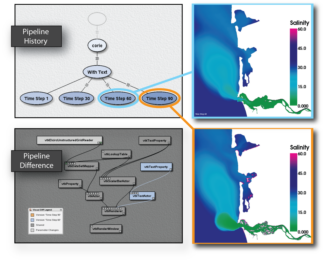
\includegraphics{VTKTextbook-38}
  \captionof*{figure}{\textit{The VisTrails multi-view visualization system.
          VisTrials enables interactive creation of visualization pipelines, maintaining the history of their evolution, optimizing their execution and allowing multiple pipelines to be compared in a spreadsheet-style layout.
          Image courtesy of SCI Institute University of Utah.}}
 \end{minipage}
\vspace{2\baselineskip}

\firstletter{I}n the previous chapter we created graphical images using simple mathematical models for lighting, viewing, and geometry. The lighting model included ambient, diffuse, and specular effects. Viewing included the effects of perspective and projection. Geometry was defined as a static collection of graphics primitives such as points and polygons. In order to describe the process of visualization we need to extend our understanding of geometry to include more complex forms. We will see that the visualization process transforms data into graphics primitives. This chapter examines the process of data transformation and develops a model of data flow for visualization systems.

\section {Overview}
Visualization transforms data into images that efficiently and accurately convey information about the data. Thus, visualization addresses the issues of \emph{transformation} and \emph{representation}.

Transformation is the process of converting data from its original form into graphics primitives, and eventually into computer images. This is our working definition of the visualization process. An example of such a transformation is the process of extracting stock prices and creating an $x-y$ plot depicting stock price as a function of time.

Representation includes both the internal data structures used to depict the data and the graphics primitives used to display the data. For example, an array of stock prices and an array of times are the computational representation of the data, while the $x-y$ plot is the graphical representation. Visualization transforms a computational form into a graphical form.

From an object--oriented viewpoint, transformations are processes in the functional model, while representations are the objects in the object model. Therefore, we characterize the visualization model with both functional models and object models.

\subsection{A Data Visualization Example}
\label{subsec:data_visualization_example}

A simple mathematical function for a quadric will clarify these concepts. The function

\begin{equation}\label{eq:4.1}
F(x,y,z) = a_0x^2 + a_1y^2 + a_2z^2 + a_3xy + a_4yz + a_5xz + a_6x + a_7y + a_8z + a9
\end{equation}
\myequations{A quadric function.}

is the mathematical representation of a quadric. Figure \ref{fig:Figure4-1a} shows a visualization of Equation \ref{eq:4.1} in the region $-1 \leqslant x, y, z \leqslant 1$. The visualization process is as follows. We sample the data on a regular grid at a resolution of $50 \times 50 \times 50$. Three
different visualization techniques are then used. On the left, we generate 3D surfaces corresponding to the function $F(x,y,z) = c$ where $c$ is an arbitrary constant (i.e., the isosurface value). In the center, we show three different planes that cut through the data and are colored by function value. On the right we show the same three planes that have been contoured with constant valued lines. Around each we place a wireframe outline.

\begin{figure}[htb]
  \begin{subfigure}[h]{0.68\linewidth}
    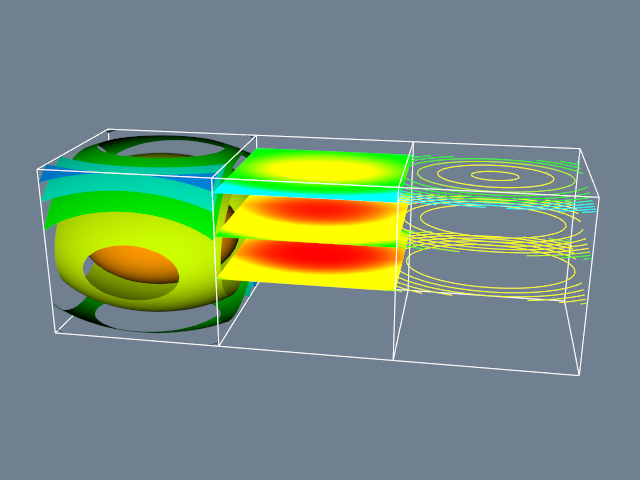
\includegraphics[width=\linewidth]{Figure4-1a}
    \caption{Quadric visualization. (\href{https://lorensen.github.io/VTKExamples/site/Cxx/Visualization/QuadricVisualization/}{QuadricVisualization.cxx} or \href{https://lorensen.github.io/VTKExamples/site/Python/Visualization/QuadricVisualization/}{QuadricVisualization.py})}
    \label{fig:Figure4-1a}
  \end{subfigure}
  \hfill
  \begin{subfigure}[h]{0.68\linewidth}
    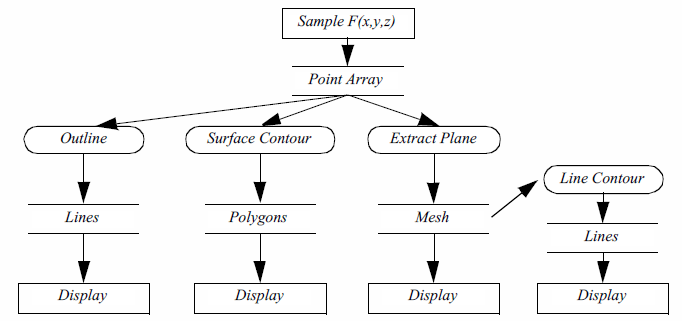
\includegraphics[width=\linewidth]{Figure4-1b}
    \caption{Functional model.}\label{fig:Figure4-1b}
  \end{subfigure}%
  \hfill
  \begin{subfigure}[h]{0.68\linewidth}
    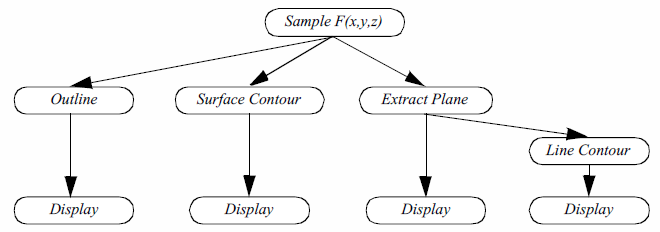
\includegraphics[width=\linewidth]{Figure4-1c}
    \caption{Visualization network.}\label{fig:Figure4-1c}
  \end{subfigure}
  \caption{Visualizing a quadric function $F(x,y,z) = c$.}\label{fig:Figure4-1}
\end{figure}

\subsection{The Functional Model}
\label{subsec:the_functional_model}
\index{functional model!in visualization|(}

The functional model in Figure \ref{fig:Figure4-1b} illustrates the steps to create the visualization. The oval blocks indicate operations (processes) we performed on the data, and the rectangular blocks represent data stores (objects) that represent and provide access to data. Arrows indicate the direction of data movement. Arrows that point into a block are inputs; data flowing out of a block indicate outputs. The blocks also may have local parameters that serve as additional input. Processes that create data with no input are called data \emph{source} objects, or simply sources. Processes that consume data with no output are called \emph{sinks} (the are also called \emph{mappers} because these processes map data to a final image or output). Processes with both an input and an output are called \emph{filters}\index{filter object}.

The functional model shows how data flows through the system. It also describes the dependency of the various parts upon one another. For any given process to execute correctly, all the inputs must be up to date. This suggests that functional models require a synchronization mechanism to insure that the correct output will be generated.
\index{functional model!in visualization|)}

\subsection{The Visualization Model}
\label{subsec:the_visualization_model}

In the examples that follow we will frequently use a simplified representation of the functional model to describe visualization processes (Figure \ref{fig:Figure4-1c}). We will not explicitly distinguish between sources, sinks, data stores, and process objects. Sources and sinks are implied based on the number of inputs or outputs. Sources will be process objects with no input. Sinks will be process objects with no output. Filters will be process objects with at least one input and one output. Intermediate data stores will not be represented. Instead we will assume that they exist as necessary to support the data flow. Thus, as Figure \ref{fig:Figure4-1c} shows, the \emph{Lines} data store that the \emph{Outline} object generates (Figure \ref{fig:Figure4-1b}) are combined into the single object \emph{Outline}. We use oval shapes to represent objects in the visualization model.

\subsubsection{The Object Model}
\index{object model!in visualization|(}

The functional model describes the flow of data in our visualization,
the object model describes which modules operate on it. But what \emph{are} the objects in the system? At first glance, we have two choices (Figure \ref{fig:Figure4-2}).

\begin{figure}[!htb]
  \centering
  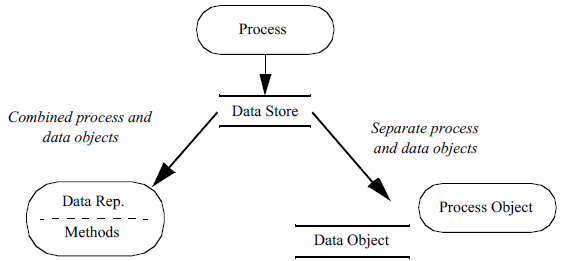
\includegraphics[width=0.8\textwidth]{Figure4-2}\\
  \caption{Object model design choices. One basic choice is to combine processes and data stores into a single object. This is the usual object--oriented choice. Another choice creates separate data objects and process objects.}\label{fig:Figure4-2}
\end{figure}

The first choice combines data stores (object attributes) with processes (object methods) into a single object. In the second choice we use separate objects for data stores and processes. There is actually a third alternative: a hybrid combination of these two choices.

The conventional object--oriented approach (our first choice above) combines data stores and processes into a single object. This view follows the standard definition that objects contain a data representation combined with procedures to operate on the data. One advantage of this approach is that the processes, which are the data visualization algorithms, have complete access to the data structures, resulting in good computational performance. But this choice suffers from several drawbacks.

\begin{itemize}

\item From a user's perspective, processes are often viewed as independent of data representation. In other words, processes are naturally viewed as objects in the system. For example, we often say we want to "contour" data, meaning creating lines or surfaces corresponding to a constant data value. To the user it is convenient to have a single contour object to operate on different data representations.

\item We must duplicate algorithm implementation. As in the previous contouring example, if we bind data stores and processes into a single object, the contour operation must be recreated for each data type. This results in duplicating code even though the implementations of an algorithm may be functionally and structurally similar. Modifying such algorithms also means modifying a large amount of code, since they are implemented across many objects.

\item Binding data stores and algorithms together results in complex, data dependent code. Some algorithms may be much more complex than the data they operate on, with large numbers of instance variables and elaborate data structures. By combining many such algorithms with a data store, the complexity of the object greatly increases, and the simple meaning of the object becomes lost.

\end{itemize}

The second choice separates the data stores and processes. That is, one set of objects represents and provides access to the data, while another set of objects implements all operations on the data. Our experience shows that this is natural to users, although it may be considered unconventional to the object--oriented purist. We also have found that the resulting code is simple, modular, and easy for developers to understand, maintain, and extend.

One disadvantage to the second choice is that the interface between data representation and process is more formal. Thus the interface must be carefully designed to insure good performance and flexibility. Another disadvantage is that strong separation of data and process results in duplicate code. That is, we may implement operations that duplicate algorithms and that cannot be considered strictly data access methods. One example of such a situation is computing data derivatives. This operation is more than simple data access, so strictly speaking it doesn't belong in the data object methods. So to compute derivatives we would have to duplicate the code each time we needed derivatives computed. (Or create a procedural library of functions or macros!)

As a result of these concerns we use the hybrid approach in the \emph{Visualization Toolkit}. Our approach is closest to the second choice described above, but we have selected a small set of critical operations that we implement within the data objects. These operations have been identified based on our experience implementing visualization algorithms. This effectively combines the first two choices to receive the maximum benefit and fewest disadvantages of each.
\index{object model!in visualization|)}

\section{The Visualization Pipeline}
\label{sec:visualization_pipeline}

In the context of data visualization, the functional model of Figure \ref{fig:Figure4-1c} is referred to as the \emph{visualization pipeline} or \emph{visualization network}. The pipeline consists of objects to represent data (data objects), objects to operate on data (process objects), and an indicated direction of data flow (arrow connections between objects). In the text that follows, we will frequently use visualization networks to describe the implementation of a particular visualization technique.

\subsection{Data Objects}
\label{subsec:data_objects}

\emph{Data objects\index{data object}} represent information. Data objects also provide methods to create, access, and delete this information. Direct modification of the data represented by the data objects is not allowed except through formal object methods. This capability is reserved for process objects. Additional methods are also available to obtain characteristic features of the data. This includes determining the minimum and maximum data values, or determining the size or the number of data values in the object.

Data objects differ depending upon their internal representation. The internal representation has significant impact on the access methods to the data, as well as on the storage efficiency or computational performance of process objects that interact with the data object. Hence, different data objects may be used to represent the same data depending on demands for efficiency and process generality.

\subsection{Process Objects}
\label{subsec:process_objects}

\emph{Process objects} operate on input data to generate output data. A process object either derives new data from its inputs, or transforms the input data into a new form. For example, a process object might derive pressure gradient data from a pressure field or transform the pressure field into constant value pressure contours. The input to a process object includes both one or more data objects as well as local parameters to control its operation. Local parameters include both instance variables or associations and references to other objects. For example, the center and radius are local parameters to control the generation of sphere primitives.

Process objects are further characterized as \emph{source objects}, \emph{filter objects}, or \emph{mapper objects}. This categorization is based on whether the objects initiate, maintain, or terminate visualization data flow.

Source objects interface to external data sources or generate data from local parameters. Source objects that generate data from local parameters are called \emph{procedural objects}. The previous example of Figure \ref{fig:Figure4-1} uses a procedural object to generate function values for the quadric function of Equation \ref{eq:4.1}. Source objects that interface to external data are called \emph{reader} objects since the external file must be read and converted to an internal form. Source objects may also interface to external data communication ports and devices. Possible examples include simulation or modelling programs, or data acquisition systems to measure temperature, pressure, or other similar physical attributes.

Filter objects\index{filter object} require one or more input data objects and generate one or more output data objects. Local parameters control the operation of the process object. Computing weekly stock market averages, representing a data value as a scaled icon, or performing union set operations on two input data sources are typical example processes of filter objects.

Mapper\index{device!mapper}\index{mapper!device}\index{mapper object} objects correspond to the sinks in the functional model. Mapper objects require one or more input data objects and terminate the visualization pipeline data flow. Usually mapper objects are used to convert data into graphical primitives, but they may write out data to a file or interface with another software system or devices. Mapper objects that write data to a computer file are termed \emph{writer}\index{device!writer} objects.

\section{Pipeline Topology}
\label{sec:pipeline_topology}

In this section we describe how to connect data and process objects to form visualization networks.

\subsection{Pipeline Connections}
\label{subsec:pipeline_connections}

The elements of the pipeline (sources, filters, and mappers) can be connected in a variety of ways to create visualization networks. However, there are two important issues that arise when we try to assemble these networks: \emph{type} and \emph{multiplicity}.

Type means the form or type of data that process objects take as input or generate as output. For example, a sphere source object may generate as output a polygonal or faceted representation, an implicit representation (e.g., parameters of a conic equation), or a set of occupancy values in a discretized representation of 3D space. Mapper objects might take as input polygonal, triangle strip, line, or point geometric representations. The input to a process object must be specified correctly for successful operation.

\begin{figure}[htb]
    \centering
	\begin{subfigure}[h]{0.48\linewidth}
        \centering
		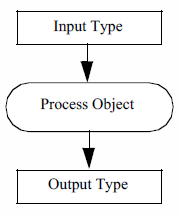
\includegraphics[width=0.56\linewidth]{Figure4-3a}
		\captionsetup{justification=centering}
		\caption{Single type system \\ \emph{Input Type = Output Type}} 
		\label{fig:Figure4-3a}
	\end{subfigure}
	\hfill
	\begin{subfigure}[h]{0.48\linewidth}
		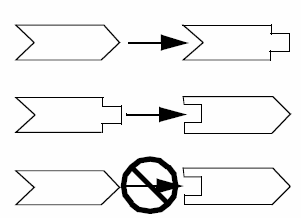
\includegraphics[width=0.96\linewidth]{Figure4-3b}
		\captionsetup{justification=centering}
		\caption{Enforced type checking}
		\label{fig:Figure4-3b}
	\end{subfigure}
	\caption{Maintaining compatible data type. (a) Single-type systems require no type checking. (b) In multiple-type systems only compatible types can be connected together.}\label{fig:Figure4-3}
\end{figure}

There are two general approaches to maintain proper input type. One approach is to design with type-less or single-type systems. That is, create a single type of data object and create filters that operate only on this one type (Figure \ref{fig:Figure4-3a}). For example, we could design a general \emph{DataSet} that represents any form of data that we're interested in, and the process objects would only input \emph{DataSets} and generate \emph{DataSets}. This approach is simple and elegant, but inflexible. Often, particularly useful algorithms (i.e., process objects) will operate only on specific types of data and generalizing them results in large inefficiencies in representation or data access. A typical example is a data object that represents structured data such as pixmaps or 3D volumes. Because the data is structured it can easily be accessed as planes or lines. However, a general representation will not include this capability since typically data is not structured.

Another approach to maintain proper input type is to design typed systems. In typed systems only objects of compatible type are allowed to be connected together. That is, more than one type is designed, but type checking is performed on the input to insure proper connection. Depending on the particular computer language, type checking can be performed at compile, link, or run time. Although type checking does insure correct input type, this approach often suffers from an explosion of types. If not careful, the designers of a visualization system may create too many types, resulting in a fragmented, hard to use and understand system. In addition, the system may require a large number of \emph{type-converter} filters. (Type-converter filters serve only to transform data from one form to another.) Carried to extremes, excessive type conversion results in computationally and memory wasteful systems.

The issue of multiplicity deals with the number of input data objects\index{multiple input} allowed, and the number of output data objects\index{multiple output} created during the operation of a process object (Figure \ref{fig:Figure4-4}). We know that all filter and mapper objects require at minimum one input data object, but in general these filters can operate sequentially across a list of input\index{fan--in}. Some filters may naturally require a specific number of inputs. A filter implementing boolean operations is one example. Boolean operations such as union or intersection are implemented on data values two at a time. However, even here more than two inputs may be defined as a recursive application of the operation to each input.

\begin{figure}[!htb]
  \centering
  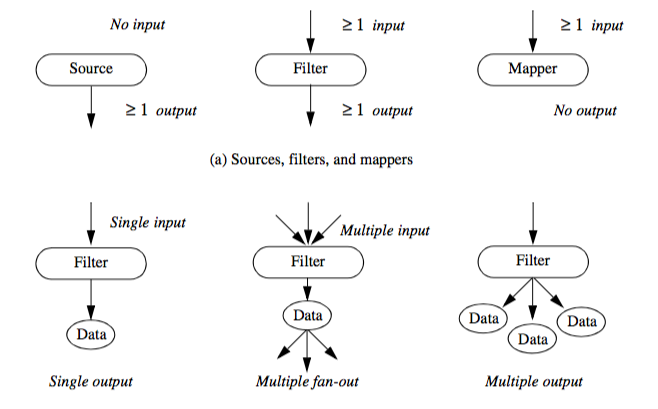
\includegraphics[width=0.8\textwidth]{Figure4-4}\\
  \caption{Multiplicity of input and output. (a) Definition of source, filter, and mapper objects. (b) Various types of input and output.}\label{fig:Figure4-4}
\end{figure}

We need to distinguish what is meant by multiplicity of output. Most sources and filters generate a single output. \emph{Multiple fan-out}\index{fan--out} occurs when an object generates an output that is used for input by more than one object. This would occur, for example, when a source object is used to read a data file, and the resulting data is used to generate a wireframe outline of the data, plus contours of the data (e.g., Figure \ref{fig:Figure4-1a}). Multiple output occurs when an object generates two or more output data objects. An example of multiple output is generating x, y, and z components of a gradient function as distinct data objects. Combinations of multiple fan-out and multiple output are possible.

\subsection{Loops}
\label{subsec:loops}

In the examples described so far, the visualization networks have been free of cycles. In graph theory these are termed directed, acyclic graphs. However, in some cases it is desirable to introduce feedback loops into our visualization networks. Feedback loops in a visualization network allow us to direct the output of a process object upstream to affect its input.

Figure \ref{fig:Figure4-5} shows an example of a feedback loop in a visualization network. We seed a velocity field with an initial set of random points. A probe filter is used to determine the velocity (and possibly other data) at each point. Each point is then repositioned in the direction of its associated vector value, possibly using a scale factor to control the magnitude of motion. The process continues until the points exit the data set or until a maximum iteration count is exceeded.

\begin{figure}[!htb]
  \centering
  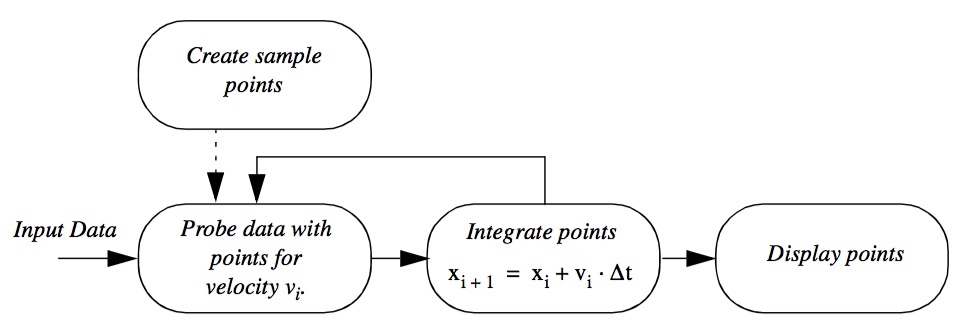
\includegraphics[width=0.8\textwidth]{Figure4-5}\\
  \caption{Looping in a visualization network. This example implements linear integration. The sample points are created to initialize the looping process. The output of the integration filter is used in place of the sample points once the process begins.}\label{fig:Figure4-5}
\end{figure}

We will discuss the control and execution of visualization networks in the next section. However, suffice it to say that loops can pose special problem in visualization networks depending on the design of the execution model. The design must insure that the loop does not enter an infinite loop or nonterminating recursive state. Typically, the number of executions of the loop is limited in order to view intermediate results. However, it is possible to execute the loop repeatedly to process data as required.

\section{Executing the Pipeline}
\label{sec:executing_pipeline}
\index{execution|(}

So far we have seen the basic elements of the visualization network and ways to connect these elements together. In this section we discuss how to control the execution of the network.

To be useful, a visualization network must process data to generate a desired result. The complete process of causing each process object to operate is called the execution of the network.

Most often the visualization network is executed more than once. For example, we may change the parameters of, or the input to, a process object. This is typically due to user interaction: The user may be exploring or methodically varying input to observe results. After one or more changes to the process object or its input, we must execute the network to generate up-to-date results.

For highest performance, the process objects in the visualization network must execute only if a change occurs to their input. In some networks, as shown in Figure \ref{fig:Figure4-6}, we may have parallel branches that need not execute if objects are modified local to a particular branch. In this figure, we see that object D and the downstream objects E and F must execute because D's input parameter is changed, and objects E and F depend on D for their input. The other objects need not execute because there is no change to their input.

We can control the execution of the network using either a demand--driven\index{demand--driven execution} or event--driven\index{event--driven execution} approach. In the demand--driven approach, we execute the network only when output is requested, and only that portion of the network affecting the result. In the event--driven approach, every change to a process object or its input causes the network to re--execute. The advantage of the event driven approach is that the output is always up to date (except during short periods of computation). The advantage of the demand--driven approach is that large numbers of changes can be processed without intermediate computation (i.e., data is processed only after the request for data is received). The demand--driven approach minimizes computation and results in more interactive visualization networks.

\begin{figure}[!htb]
  \centering
  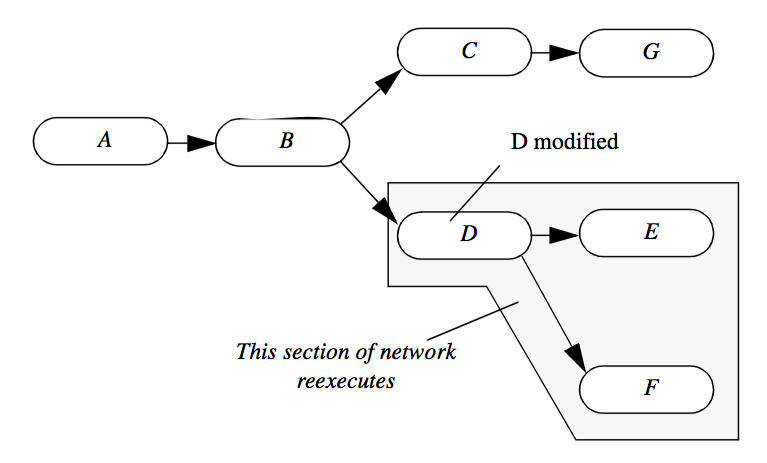
\includegraphics[width=0.8\textwidth]{Figure4-6}\\
  \caption{Network execution. Parallel branches need not execute.}\label{fig:Figure4-6}
\end{figure}

The execution of the network requires synchronization between process objects. We want to execute a process object only when all of its input objects are up to date. There are generally two ways to synchronize network execution: explicit or implicit control (Figure \ref{fig:Figure4-7}).

\subsection{Explicit Execution}
\label{subsec:explicit_execution}
\index{execution!explicit|(}\index{explicit execution|(}

Explicit control means directly tracking the changes to the network, and then directly controlling the execution of the process objects based on an explicit dependency analysis. The major characteristic of this approach is that a centralized \emph{executive} is used to coordinate network execution. This executive must track changes to the parameters and inputs of each object, including subsequent changes to the network topology (Figure \ref{fig:Figure4-7a}).

The advantage of this approach is that synchronization analysis and update methods are local to the single executive object. In addition, we can create dependency graphs and perform analysis of data flow each time output is requested. This capability is particularly important if we wish to decompose the network for parallel computing or to distribute execution across a network of computers.

The disadvantage of the explicit approach is that each process object becomes dependent upon the executive, since the executive must be notified of any change. Also, the executive cannot easily control execution if the network execution is conditional, since whether to execute or not depends on the local results of one or more process objects. Finally, a centralized executive can create non-scalable bottlenecks in parallel computing environments.

The explicit approach may be either demand-driven or event-driven. In the event-driven approach, the executive is notified whenever a change to an object occurs (typically in response to a user--interface event), and the network is immediately executed. In the demand-driven approach, the executive accumulates changes to object inputs and executes the network based on explicit user demand.

\begin{figure}[htb]
    \centering
	\begin{subfigure}[h]{0.48\linewidth}
        \centering
		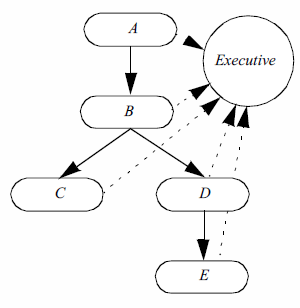
\includegraphics[width=0.96\linewidth]{Figure4-7a}
		\captionsetup{justification=centering}
        \captionsetup{singlelinecheck=off}
		\caption{Explicit \\ 
        \begin{enumerate}
        \item A parameter modified
        \item Executive performs dependency analysis
        \item Executive executes necessary modules in order A--B--C--D--E
        \end{enumerate}} 
		\label{fig:Figure4-7a}
	\end{subfigure}
	\hfill
	\begin{subfigure}[h]{0.48\linewidth}
		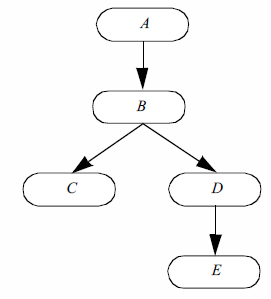
\includegraphics[width=0.96\linewidth]{Figure4-7b}
		\captionsetup{justification=centering}
        \captionsetup{singlelinecheck=off}
		\caption{Implicit \\ 
        \begin{enumerate}
        \item A parameter modified
        \item E output requested
        \item Chain E--D--B--A back propagates \texttt{Update()} method
        \item Chain A--B--D--E executes via \texttt{RequestData()} method
        \end{enumerate}} 
		\label{fig:Figure4-7b}
	\end{subfigure}
	\caption{Explicit and implicit network execution.}\label{fig:Figure4-7}
\end{figure}


The explicit approach with a central executive is typical of many commercial visualization systems such as AVS\index{AVS}, Iris Explorer\index{Iris Explorer}, and IBM Data Explorer\index{Data Explorer}. Typically these systems use a visual-programming interface to construct the visualization network. Often these systems are implemented on parallel computers, and the ability to distribute computation is essential.
\index{execution!explicit|)}\index{explicit execution|)}

\subsection{Implicit Execution}
\label{subsec:implicit_execution}
\index{execution!implicit|(}\index{implicit execution|(}

Implicit control means that a process object executes only if its local input or parameters change (Figure 4-7 \ref{fig:Figure4-7b}). Implicit control is implemented using a two-pass process. First, when output is requested from a particular object, that object requests input from its input objects. This process is recursively repeated until source objects are encountered. The source objects then execute if they have changed or their external inputs have changed. Then the recursion unwinds as each process object examines its inputs and determines whether to execute. This procedure repeats until the initial requesting object executes and terminates the process. These two steps are called the \emph{update} and \emph{execution} passes.

Implicit network execution is naturally implemented using \emph{demand-driven} control. Here network execution occurs only when output data is requested. Implicit network execution may also be event-driven if we simply request output each time an appropriate event is encountered (such as change to object parameter).

\begin{figure}[!htb]
  \centering
  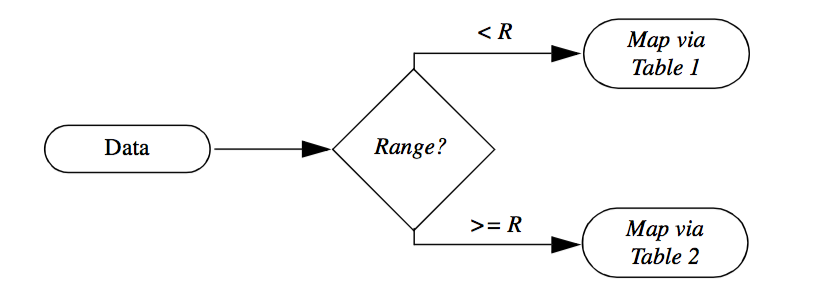
\includegraphics[width=0.8\textwidth]{Figure4-8}\\
  \caption{Examples of conditional execution. Depending upon range, data is mapped through different color lookup tables.}\label{fig:Figure4-8}
\end{figure}

The primary advantage of the implicit control scheme is its simplicity. Each object only need keep track of its internal modification time. When output is requested, the object compares its modification time with that of its inputs, and executes if out of date. Furthermore, process objects need only know about their direct input, so no global knowledge of other objects (such as a network executive) is required.

The disadvantage of implicit control is that it is harder to distribute network execution across computers or to implement sophisticated execution strategies. One simple approach is to create a queue that executes process objects in order of network execution (possibly in a distributed fashion). Of course, once a central object is introduced back into the system, the lines between implicit and explicit control are blurred.
\index{execution!implicit|)}\index{implicit execution|)}

\subsection{Conditional Execution}
\label{subsec:conditional_execution}
\index{conditional execution|(}\index{execution!conditional|(}

Another important capability of visualization networks is conditional execution. For example, we may wish to map data through different color lookup tables depending upon the variation of range in the data. Small variations can be amplified by assigning more colors within the data range, while we may compress our color display by assigning a small number of colors to the data range (Figure \ref{fig:Figure4-8}). 

The conditional execution of visualization models (such as that shown Figure \ref{fig:Figure4-1c}) can be realized in principle. However, in practice we must supplement the visualization network with a conditional language to express the rules for network execution. Hence, conditional execution of visualization networks is a function of implementation language. Many visualization systems are programmed using the visual programming style. This approach is basically a visual editor to construct data flow diagrams directly. It is difficult to express conditional execution of networks using this approach. Alternatively, in a procedural programming language, conditional execution of networks is straightforward. We defer discussions of the topic until ``Putting It All Together'' on page \pageref{sec:chap04.putting_it_all_together}.
\index{conditional execution|)}\index{execution!conditional|)}
\index{execution|)}

\section{Memory and Computation Trade-off}
\label{sec:memory_computation_trade-off}

Visualization is a demanding application, both in terms of computer memory and computational requirements. Data streams on the order of one megabyte to one gigabyte are not uncommon. Many visualization algorithms are computationally expensive, in part due to input size, but also due to the inherent algorithm complexity. In order to create applications that have reasonable performance, most visualization systems have various mechanisms to trade off memory and computation costs.

\begin{figure}[!htb]
  \centering
  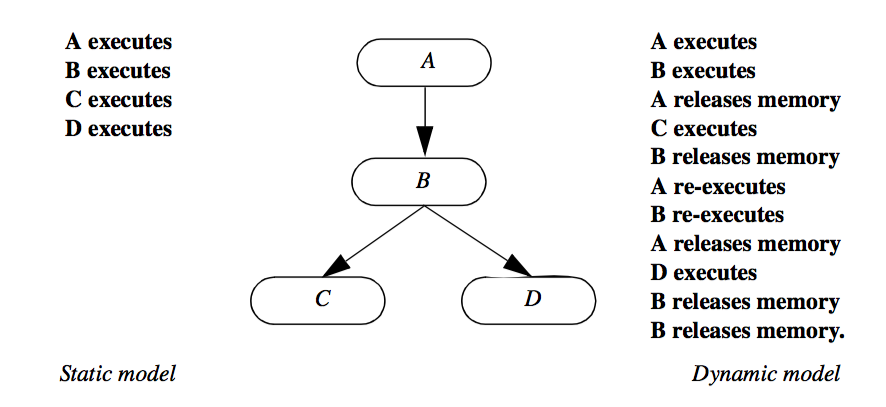
\includegraphics[width=0.8\textwidth]{Figure4-9}\\
  \caption{Comparison of static versus dynamic memory models for typical network. Execution begins when output is requested from objects \emph{C} and \emph{D}. In more complex dynamic models, we can prevent \emph{B} from executing twice by performing a more thorough dependency analysis image.}\label{fig:Figure4-9}
\end{figure}

\subsection{Static and Dynamic Memory Models}
\label{subsec:static_dynamic_memory_models}
\index{memory model!dynamic|(}\index{memory model!static|(}

Memory and computation trade-offs are important performance issues when executing visualization networks. In the networks presented thus far, the output of a process object is assumed to be available to downstream process objects at all times. Thus, network computation is minimized. However, the computer memory requirement to preserve filter output can be huge. Networks of only a few objects can tie up extensive computer memory resources.

An alternative approach is to save intermediate results only as long as they are needed by other objects. Once these objects finish processing, the intermediate result can be discarded. This approach results in extra computation each time output is requested. The memory resources required are greatly reduced at the expense of increased computation. Like all trade-offs, the proper solution depends upon the particular application and the nature of the computer system executing the visualization network.

We term these two approaches as \emph{static} and \emph{dynamic}\index{dynamic memory model} memory models. In the static model intermediate data is saved to reduce overall computation. In the dynamic model intermediate data is discarded when it is no longer needed. The static model serves best when small, variable portions of the network reexecute, and when the data sizes are manageable by the computer system. The dynamic model serves best when the data flows are large, or the same part of the network executes each time. Often, it is desirable to combine both the static and dynamic models into the same network. If an entire leg of the network must execute each time, it makes no sense to store intermediate results, since they are never reused. On the other hand, we may wish to save an intermediate result at a branch point in the network, since the data will more likely be reused. A comparison of the static and dynamic memory model for a specific network is shown in Figure \ref{fig:Figure4-9}.

\begin{figure}[!htb]
  \centering
  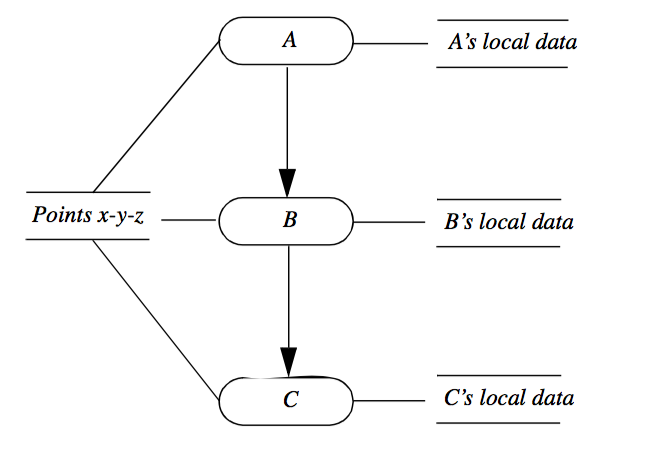
\includegraphics[width=0.8\textwidth]{Figure4-10}\\
  \caption{Reference counting to conserve memory resource. Each filter \emph{A}, \emph{B}, and \emph{C} shares a common point representation. Other data is local to each object.}\label{fig:Figure4-10}
\end{figure}

As this figure shows, the static model executes each process object only once, storing intermediate results. In the dynamic model, each process object releases memory after downstream objects complete execution. Depending upon the implementation of the dynamic model, process object \emph{B} may execute once or twice. If a thorough dependency analysis is performed, process \emph{B} will release memory only after both objects \emph{C} and \emph{B} execute. In a simpler implementation, object \emph{B} will release memory after \emph{C} and subsequently, \emph{D} executes.
\index{memory model!dynamic|)}\index{memory model!static|)}

\subsection{Reference Counting and Garbage Collection}
\label{subsec:reference_counting_garbage_collection}
\index{memory management!reference counting|(}

Another valuable tool to minimize memory cost is to share storage using reference counting. To use reference counting, we allow more than one process object to refer to the same data object and keep track of the number of references. For example, assume that we have three objects \emph{A}, \emph{B}, and \emph{C} that form a portion of a visualization network as shown in Figure \ref{fig:Figure4-10}. Also assume that these objects modify only part of their input data, leaving the data object that specifies \emph{x-y-z} coordinate position unchanged. Then to conserve memory resources we can allow the output of each process object to refer to the single data object representing these points. Data that is changed remains local to each filter and is not shared. It is only when the reference count goes to zero that the object is deleted.

Garbage collection is an alternative memory management strategy that is not well suited to visualization applications. The garbage collection process is automatic; it attempts to reclaim memory used by objects that will never again be accessed by the running application. While convenient due to its automated nature, in general garbage collection introduces overhead that may inadvertently introduce pauses into software execution at inopportune times (during an interactive process). Of more concern, however, is that released, unused memory may not be reclaimed by the system until some time after the last reference to the memory is dropped, and in visualization pipelines this memory may be too large to leave around for any length of time. That is, in some applications if memory usage in a filter is not released immediately, downstream filters may not have enough memory resource available to them to successfully execute.
\index{memory management!reference counting|)}

\section{Advanced Visualization Pipeline Models}
\label{sec:advanced_visualization_pipeline_models}

The preceding sections have provided a general framework for the implementation of a useful visualization pipeline model. However, there are several advanced capabilities that complex applications often require. These capabilities are driven by deficiencies in the simpler design described previously. The principle drivers for developing advanced models include: processing unknown dataset types, managing complex execution strategies including processing pieces of data, and extending the visualization pipeline to propagate new information. These concerns are discussed in the following three sections.

\subsection{Processing Unknown Dataset Types}
\label{subsec:processing_unknown_dataset_types}

There exist data files and data sources where the type of dataset represented by the file or source is unknown until run-time. For example, consider a general purpose VTK reader that can read any type of VTK data file. Such a class is convenient because the user need not concern himself with the type of dataset, instead the user may want to set up a single pipeline that processes whatever type is found. As indicated by Figure \ref{fig:Figure4-3}, such an approach works well if the system is of a single dataset type, however in practice, and due to performance/efficiency concerns, there typically exist many different types of data in a visualization system. The other alternative shown in Figure \ref{fig:Figure4-3} is enforced type checking. However, in situations like the reader example described above, it is not possible to enforce type checking at compile-time because the type is determined by the data. As a result, type checking must be performed at run-time.

Run-time type checking of a multiple dataset type visualization system requires that the data passed between filters is a generic dataset container (i.e., it appears like a single type but contains the actual data and methods to determine what type of data it is). Run-time type checking has the advantage of flexibility, but the trade-off is that a pipeline may not execute properly until the program executes. For example, a generic pipeline may be designed that can process structured data (see ``Types of Datasets''on page \pageref{sec:types_of_datasets}), but the data file may contain unstructured data. In this case, the pipeline will be unable to execute at run-time, producing empty output. Thus pipelines designed to process any type of data must be carefully assembled to create robust applications.

\subsection{Extending the Data Object Representation}
\label{subsec:extending_data_object_representation}

As described earlier in this chapter, a pipeline consists of data objects that are operated on by process objects. Further, because the process objects are separate from the data objects on which they operate, there is necessarily an expected interface through which these objects exchange information. Defining this interface has the side effect of cementing the data representation, implying that it is difficult to extend it without modifying the corresponding interface, and hence all the classes that depend on the interface (of which there are many). Fortunately what tends to change is not the basic data representations (these are generally well established), rather the metadata associated with the dataset itself changes. (In the context of visualization, metadata are data that describe datasets.) While it is feasible to represent new datasets by creating new classes (since the addition of new dataset types occurs infrequently); the diversity of metadata precludes creating new classes because the resulting explosion of data types, and the potential change to programming interfaces, would adversely affect the stability of the visualization system. Hence a general mechanism to support metadata is required. Packaging metadata into a generic container that contains both the dataset andcmetadata is a obvious design, and is compatible with the design described in the previous section.

Examples of metadata include time step information, data ranges or other data characteristics, acquisition protocols, patient names, and annotation. In an extensible visualization pipeline, a specific data reader (or other data source) may read such information and associate it with the output data that it produces. While many filters may ignore the metadata, they can be configured to pass the information along the pipeline. Alternatively, a pipeline sink (or mapper) may request that specific metadata be passed through the pipeline so it can be processed appropriately. For example, a mapper may request annotations, and if available, place them on the final image.

\subsection{Managing Complex Execution Strategies}
\label{subsec:managing_complex_execution_strategies}

In real-world applications the pipeline design described thus far may not adequately support complex execution strategies, or may fail to execute successfully when data sizes become large. In the next sections we address these issues by considering alternative design possibilities.

\textbf{Large Data}. Previous discussions relative to the visualization pipeline have assumed that the size of a particular dataset does not exceed the total memory resource of a computer system. However, with modern dataset sizes pushing into the terabyte and even petabyte range, a typical desktop computer system is incapable of processing such datasets. Thus alternative strategies must be adopted when processing large data. One such approach is based on breaking data into pieces, and then \emph{streaming} the pieces through the visualization pipeline \cite{Martin01}. Figure \ref{fig:Figure4-11} illustrates how a dataset can be divided into pieces.

\begin{figure}[!htb]
  \centering
  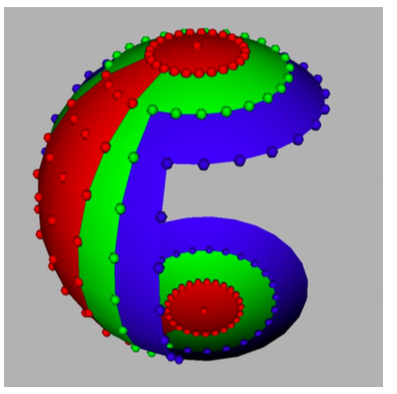
\includegraphics[width=0.8\textwidth]{Figure4-11}\\
  \caption{Dividing a sphere into a piece (red) with ghost level cells and points (blue and green).}\label{fig:Figure4-11}
\end{figure}

Streaming data through a visualization pipeline offers two major benefits. The first is that visualization data that would not normally fit into memory can be processed. The second is that visualizations can be run with a smaller memory footprint resulting in higher cache hits, and little or no swapping to disk. To realize these benefits the visualization software must support breaking the dataset into pieces and correctly processing those pieces. This requires that the dataset and the algorithms that operate on it are \emph{separable}, \emph{mappable}, and \emph{result invariant} as described in the following \cite{Law99}.

\begin{enumerate}
\item \textbf{Separable}. The data must be separable. That is, the data can be broken into pieces. Ideally, each piece should be coherent in geometry, topology, and/or data structure. The separation of the data should be simple and efficient. In addition, the algorithms in this architecture must be able to correctly process pieces of data.

\item \textbf{Mappable}. In order to control the streaming of the data through a pipeline, we must be able to determine what portion of the input data is required to generate a given portion of the output. This allows us to control the size of the data through the pipeline, and configure the algorithms.

\item \textbf{Result Invariant}. The results should be independent of the number of pieces, and independent of the execution mode (i.e., single- or multi-threaded). This means proper handling of boundaries and developing algorithms that are multi-thread safe across pieces that may overlap on their boundaries.
\end{enumerate}

Separating data into pieces is relatively straightforward if the data is structured, i.e., topologically regular (see ``Types of Datasets'' on page \pageref{sec:types_of_datasets}). Such datasets can be topological described by a rectangular extent in a regularly $x-y-z$ subdivided cubical domain (see Figures \ref{fig:Figure5-7}(a)-(c)). However, if the data is unstructured (e.g. a mesh of triangles or polygons), then specifying pieces is difficult. Generally an unstructured extent is defined by grouping adjacent data (e.g., cells) into pieces, and then addressing each piece using a $N$ of $M$ notation, where $N$ is the $n$-th piece out of a total of $M$ pieces. The exact organizational structure of a piece is left unspecified and depends on the particular application and algorithm used to group the data.

To satisfy the third requirement of results invariancy, processing pieces also requires the ability to generate boundary data, or \emph{ghost levels}\index{ghost levels!pipeline!ghost levels}. Boundary information is necessary when information from the neighbors of a piece is needed to perform a computation. For example, gradient calculations or boundary analysis (e.g., do I have a cell face neighbor?) require one level of boundary information. In rare cases, two or more levels are required. Figure \ref{fig:Figure4-11} illustrates boundary cells and points corresponding to the central red piece of the sphere.

Finally, it should be noted that the ability to divide data into pieces for streaming is exactly the same capability required for data parallel processing. In such methods, data is subdivided and sent to different processors to be operated on in parallel. Boundary information may also be required to perform certain computations. Parallel processing has the added complexity that the data must be communicated to processors (in the case of distributed computing) or mutual exclusion (i.e., mutexing) must be employed to avoid simultaneous write operations. Thus streaming and parallel processing are complementary technologies used in large data computing.

\subsubsection{Complex Execution Strategies}
\label{subsubsec:complex_execution_strategies}

In many cases the simple execution model of Figure \ref{fig:Figure4-7b} is not suitable for complex data processing tasks. For example, as discussed in the previous section, streaming data is a complex execution strategy required when a dataset becomes too large to fit into memory, or when parallel computing is used. In some cases event-driven (see ``Executing the Pipeline''on page \pageref{sec:executing_pipeline}) or ``push'' pipelines (i.e., those that receive data and push the data through the pipeline for processing) may be preferred. Finally, there exist hierarchical data structures such as multi-block or adaptive mesh refinement (AMR) \cite{Berger84} grids. Processing such datasets in a pipeline requires hierarchical traversal as filters process each block in the grid (an advanced research topic in the visualization field and not covered in this edition of the book).

Addressing these requirements implies that the execution model must be extended. Thus we revisit the object--oriented design in the next section.

\subsubsection{object--oriented Design Revisited}
\label{subsubsec:object_oriented_design_revisited}

Figure \ref{fig:Figure4-2} illustrates two choices relative to the design of the visualization object model. The first choice, which was discarded, was to combine data and operations on the data into a single object, a typical object--oriented design pattern. The second choice, which was advocated, was to create a design consisting of two classes --- data objects and process objects --- which were then combined into visualization pipelines. While this second strategy works well for simple pipelines, when complex execution strategies are introduced, this design begins to break down. This is because the execution strategy is necessarily, and implicitly, distributed across the data objects and process objects; there is no explicit mechanism to implement a particular strategy. Thus the design is problematic because new strategies cannot be introduced without modifying the interface to both the data and process objects. Good design demands that the execution strategy is separated from the data objects and process objects. The benefits of such a design include reducing the complexity of the data and process objects, encapsulating execution strategies, performing run-time type checking (see ``Processing Unknown Dataset Types'' on page \pageref{subsec:processing_unknown_dataset_types}) and even managing metadata (see ``Extending the Data Object Representation''on page  \pageref{subsec:extending_data_object_representation}).

As the execution model becomes more complex, execution strategies are separated from the data and process objects as separate classes.

\begin{wrapfigure}{r}{0.4\textwidth}
  \centering
  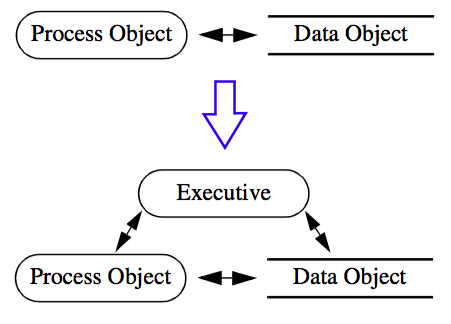
\includegraphics[width=0.96\textwidth]{Figure4-12}\\
  \caption{As the execution model becomes more complex, execution strategies are separated from the data and process objects as separate classes.}\label{fig:Figure4-12}
\end{wrapfigure}

The advanced design re-introduces the notion of an executive (see ``Executing the Pipeline'' on page \pageref{sec:executing_pipeline}). However, the design differs from that of Figure \ref{fig:Figure4-7}. As that figure illustrated, a single, centralized executive introduces dependencies into the pipeline that will not scale as pipeline complexity increases, or in parallel processing applications. In the advanced design, we assume \emph{multiple} executives, typically one per filter. In  some cases the executive may control multiple filters. This is particularly useful if the filters are interdependent or complex execution strategies are required. Different classes of executive can implement different execution strategies, for example a demand-driven, streaming pipeline is one such strategy. Other important classes include executives that coordinate the execution of filters on composite datasets.

Figure \ref{fig:Figure4-12} is a high-level view of the executive and its relationship to data and process objects. In ``Pipeline Design and Implementation'' on page \pageref{subsec:pipeline_design_implementation} the design is explored in more detail.

\section{Programming Models}
\label{sec:programming_models}

Visualization systems are by their very nature designed for human interaction. As a result they must be easy to use. On the other hand, visualization systems must readily adapt to new data, and must be flexible enough to allow rapid data exploration. To meet these demands, a variety of programming models have been developed.

\subsection{Visualization Models}
\label{subsec:visualization_models}

At the highest level are applications. Visualization applications have finely tailored user-interfaces that are specific to an application area, e.g., fluid flow visualization. Applications are the easiest to use, but are the least flexible. It is very difficult or impossible for the user to extend applications into a new domain because of inherent logistical issues. Commercial turn-key visualization software is generally considered to be application software.

At the opposite end of the spectrum are programming libraries. A conventional programming library is a collection of procedures that operate on a library-specific data structure. Often these libraries are written in conventional programming languages such as C or FORTRAN. These offer great flexibility and can be easily combined with other programming tools and techniques. Programming libraries can be extended or modified by the addition of user-written code. Unfortunately, the effective use of programming libraries requires skilled programmers. Furthermore, non graphics/visualization experts cannot easily use programming libraries because there is no notion of how to fit (or order) the procedures together correctly. These libraries also require extensive synchronization schemes to control execution as input parameters are varied.

Many visualization systems lie between these two extremes. These typically use a \emph{visual programming} approach to construct visualization networks. The basic idea is to provide graphical tools and libraries of modules or process objects. Modules may be connected subject to input/output type constraints, using simple graphical layout tools. In addition, user interface tools allow association of interface widgets with object input parameters. System execution is generally transparent to the user by way of an internal execution executive.

\subsection{Alternative Visual Programming Models}
\label{subsec:alternative_visual_programming_models}

There are two other graphics and visualization programming models that bear mentioning. These are \emph{scene graphs} and the \emph{spreadsheet} model. 

Scene graphs are typically found in 3D graphics systems such as Open Inventor\index{OpenInventor} \cite{Wernecke94}. Scene graphs are acyclic tree-structures that represent objects, or nodes, in an order defined by the tree layout. The nodes may be geometry (called shape nodes), graphics properties, transformations, manipulators, lights, cameras, and so forth, that define a complete scene. The parent/child relationship controls how properties and transformations are applied to the nodes as they are rendered, or how the objects relate to other objects in the scene (e.g., which objects the lights shine on). Scene graphs are not used to control the execution of a visualization pipeline, rather they are used to control the rendering process. Scene graphs and visualization pipelines may be used together in the same application. In such a case the visualization pipeline is the generator of the shape nodes, and the scene graph controls the rendering of the scene including the shapes.

Scene graphs have found wide use in the graphics community because of their ability to compactly and graphically represent a scene. In addition, scene graphs have been popularized by their recent use in Web tools such as VRML and Java3D. See Chapter 11: \nameref{chap:visualization_web} for more information.

Another recently introduced technique for visual programming is the spreadsheet technique of Levoy \cite{Levoy94}. In the spreadsheet model, we arrange operations on a regular grid similar to the common electronic accounting spreadsheets. The grid consists of rows and columns of cells, where each cell is expressed as a computational combination of other cells. The combination is expressed for each cell by using a simple programming language to add, subtract, or perform other more complex operations. The result of the computation (i.e., a visual output) is displayed in the cell. A recent extension to the spreadsheet approach is exemplified by VisTrails \cite{Bavoil05}, a system that enables interactive multiple-view visualizations by simplifying the creation and maintenance of visualization pipelines, and by optimizing the execution of the pipelines. VisTrials has the further benefit that it tracks changes to the visualization pipeline so that it is straightforward to create extensive design studies.

Although visual programming systems are widely successful, they suffer two drawbacks. First, they are not as tailored as an application and require extensive programming, albeit visual, to be so. Second, visual programming is too limited for detailed control, so constructing complex low-level algorithms and user-interfaces is not feasible. What is required is a visualization system that provides the ``modularity'' and automatic execution control of a visual system, and the low-level programming capability of a programming library. Object--oriented systems have the potential to provide these capabilities. Carefully crafted object libraries provide the ease of use of visual systems with the control of programming libraries. That is a major goal of the described in this text.

\section{Data Interface Issues}
\label{sec:data_interface_issues}
\index{interfacing to data|(}

At this point in the text you may be wondering how to apply a visualization pipeline towards your own data. The answer depends on the type of data you have, preferences in programming style, and required complexity. Although we have not yet described particular types of data (we will in the next chapter), there are two general approaches you may wish to consider when interfacing your data to a visualization system: a programming interface and an application interface.

\subsection{Programming Interface}
\label{subsec:programming_interface}
\index{interfacing to data!programming interface|(}

The most powerful and flexible approach is to directly program your application to read, write, and process data. There is almost no limit to what you can achieve using this approach. Unfortunately, in a complex system like VTK this requires a level of expertise that may be beyond your time budget to obtain. (If you are interested in this approach using VTK, you'll have to become familiar with the objects in the system. You will also want to refer to the Doxygen-generated manual pages --- on-line at \href{https://www.vtk.org}{https://www.vtk.org} or CD-ROM. The companion text \emph{The VTK User's Guide} is also helpful.)

Typical applications requiring a programming interface are interfacing to data files that are not currently supported by the system or generating synthetic data (e.g., from a mathematical relationship) where no data file is available. Also, sometimes it is useful to directly code your data in the form of a program, and then execute the program to visualize the results. (This is exactly what many of the VTK examples do.)

In general, programming a complex system such as VTK is a difficult undertaking because of the initial learning curve. There are, however, simpler ways to interface to data. While skilled developers may be required to create sophisticated applications, the points of an object--oriented toolkit like VTK is that it provides many of the pieces required to interface to common data forms. Thus focusing on those objects that import and export data is a good start towards interfacing with data. In VTK, these objects are known as readers, writers, importers and exporters.
\index{interfacing to data!programming interface|)}

\subsubsection{File Interface (Readers / Writers)}
\label{subsubsec:file_interface_readers_writers}
\index{interfacing to data!readers and writers|(}

In this chapter we saw that readers are source objects, and writers are mappers. What this means from a practical point of view is that readers will ingest data from a file, create a data object, and then pass the object down the pipeline for processing. Similarly, writers ingest a data object and then write the data object to a file. Thus, readers and writers will interface to your data well if VTK supports your format, \emph{and} you only need to read or write a \emph{single} data object. If your data file format is not supported by the system, you will need to interface to your data via a general programming interface described above. Or, if you wish to interface to a collection of objects, you will probably want to see whether an exporter or importer object (described in the next section) exists to support your application.

Examples of readers include vtkSTLReader (read stereo-lithography files) and vtkBYUReader (read MOVIE.BYU format data files). Similarly the objects vtkSTLWriter and vtkBYUWriter can be used to write data files. To see which readers and writers are supported by VTK, see \emph{The VTK User's Guide} or refer to the Web pages at \href{https://www.vtk.org}{https://www.vtk.org} for the current Doxygen manual pages.
\index{interfacing to data!readers and writers|)}

\subsubsection{File Interface (Importers / Exporters)}
\label{subsubsec:file_interface_importers_exporters}
\index{exporters|(}\index{exporter!interfacing to data|(}\index{importer!interfacing to data|(}\index{interfacing to data!importers and exporters|(}

\emph{Importers}\index{importers} and \emph{exporters} are objects in the system that read or write data files consisting of more than one object. Typically importers and exporters are used to save or restore an entire scene (i.e., lights, cameras, actors, data, transformations, etc.). When an importer is executed, it reads one or more files and may create several objects. For example, in VTK the vtk3DSImporter imports a \emph{3D Studio} file and creates a rendering window, renderer, lights, cameras, and actors. Similarly, the vtkVRMLExporter creates a VRML file given a VTK render window. The VRML file contains cameras, lights, actors, geometry, transformations, and the like, indirectly referred to by the rendering window provided.

In the \emph{Visualization Toolkit}, there are several importers and exporters. To see which importers and exporters are supported by VTK, see \emph{The VTK User's Guide}. You may also want to check the Web pages at \href{https://www.vtk.org}{https://www.vtk.org} for the current Doxygen manual pages. If the exporter you are looking for does not exist, you will have to develop your own using the programming interface.

\begin{figure}[htb]
  \begin{subfigure}[h]{0.48\linewidth}
    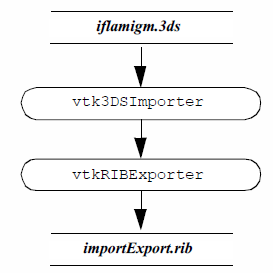
\includegraphics[width=0.96\linewidth]{Figure4-13a}
    \caption*{}
    \label{fig:Figure4-13a}
  \end{subfigure}
  \hfill
  \begin{subfigure}[h]{0.48\linewidth}
    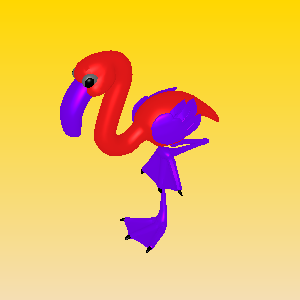
\includegraphics[width=0.96\linewidth]{Figure4-13b}
    \caption*{See:  \href{https://lorensen.github.io/VTKExamples/site/Cxx/IO/3DSImporter/}{3DSImporter.cxx} and \href{https://lorensen.github.io/VTKExamples/site/Python/IO/3DSImporter/}{3DSImporter.py}})
    \label{fig:Figure4-13b}
  \end{subfigure}
  \hfill
  \begin{subfigure}[h]{0.96\linewidth}{Figure4-13c}
  \begin{lstlisting}[language=TCL,  caption={}, numbers=none, frame=none]
    # import from 3d Studio
    vtk3DSImporter importer
      importer ComputeNormalsOn
      importer SetFileName "$VTK_DATA_ROOT/Data/iflamigm.3ds"
      importer Read
    # export to rib format
    vtkRIBExporter exporter
      exporter SetFilePrefix importExport
      exporter SetRenderWindow [importer GetRenderWindow]
      exporter BackgroundOn
      exporter Write
    \end{lstlisting} 
    \caption*{}
    \label{fig:Figure4-13c}
  \end{subfigure}
  \caption{Importing and exporting files in VTK. An importer creates a vtkRenderWindow that describes the scene. Exporters use an instance of vtkRenderWindow to obtain a description of the scene.}\label{fig:Figure4-13}
\end{figure}

Figure \ref{fig:Figure4-13} shows an image created from a \emph{3D Studio} model and saved as a \emph{Renderman} RIB file.
\index{exporters|)}\index{exporter!interfacing to data|)}\index{importer!interfacing to data|)}\index{interfacing to data!importers and exporters|)}

\subsection{Application Interface}
\label{subsec:application_interface}
\index{interfacing to data!application|(}

The majority of users interface to their data by using an existing application. Rather than programming pipelines or writing their own readers and writers, users acquire an application that suits their particular visualization needs. Then to interface to their data, users simply identify the reader, writer, importer, and/or exporter that can successfully process it. In some cases, users may have to modify the program used to generate the data so that it exports it in a standard data format. The advantage of using existing applications is that the user interface and pipeline are pre-programmed, insuring that the user can focus on their data, rather than expending the significant resources required to write visualization programs. The disadvantage of using existing applications is that necessary features are often missing, and applications typically lack the flexibility that a general purpose tool can provide.

\begin{figure}[htb]
  \begin{subfigure}[h]{0.48\linewidth}
    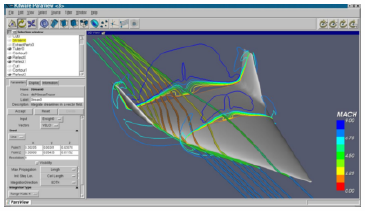
\includegraphics[width=0.96\linewidth]{Figure4-14a}
    \caption{Paraview parallel visualization application}
    \label{fig:Figure4-14a}
  \end{subfigure}
  \hfill
  \begin{subfigure}[h]{0.48\linewidth}
    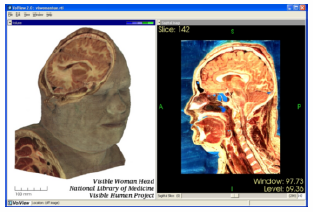
\includegraphics[width=0.96\linewidth]{Figure4-14b}
    \caption*{VolView volume rendering application}
    \label{fig:Figure4-14b}
  \end{subfigure}
  \caption{The choice of an appropriate visualization application depends on the type of dataset(s) it must support, required interaction techniques, rendering capabilities, and support for large data, including parallel processing. While both applications above are built using the VTK visualization toolkit, they provide very different user experiences. ParaView (\href{https://www.paraview.org/}{https://www.paraview.org/}) is a general purpose visualization system that can process large data in a distributed, parallel environment (as well as on single processor systems), with the ability to display on a Cave or tiled display. VolView (\href{https://www.kitware.com/volview/}{https://www.kitware.com/volview/}) focuses on volumetric and image data and uses multi-threading and sophisticated level-of-detail methods to achieve interactive performance.}\label{fig:Figure4-14}
\end{figure}

Selecting the right application is not always simple. The application must support the correct dataset types, and support suitable rendering devices, for example generating images on large displays \cite{Humphreys99} or in a Cave \cite{CruzNeira93} environment. In some cases user interaction is required, and demands on parallel processing or data handling capacities further complicates the selection. For example, while a general purpose tool like ParaView (Figure \ref{fig:Figure4-14a}) can be used to visualize most types of data, including providing support for large data and parallel computing, a specialized tool such as VolView (Figure \ref{fig:Figure4-14}(b) )may be better suited for a particular type task such as viewing medical data shown in the figure. It is imperative that users have a familiarity with the visualization process if they are to successfully choose the right application for their data.
\index{interfacing to data!application|)}
\index{interfacing to data|)}

\section{Putting It All Together}
\label{sec:chap04.putting_it_all_together}

In the previous sections we have treated a variety of topics relating to the visualization model. In this section we describe the particular implementation details that we have adopted in the \emph{Visualization Toolkit}.

\subsection{Procedural Language Implementation}
\label{subsec:procedural_language_implementation}

The \emph{Visualization Toolkit} is implemented in the procedural language C++. Automated wrapping technology creates language bindings to the Python, Tcl and Java interpretive programming languages \cite{King03}. The class library contains data objects, filters (i.e., process objects) and executives to facilitate the construction of visualization applications. A variety of supporting abstract super-classes are available to derive new objects including data objects and filters. The visualization pipeline is designed to connect directly to the graphics subsystem described in the previous chapter. This connection is via VTK's mappers, which are the sinks of the pipeline and interface to the VTK's actors.

A visual programming interface could be (and has been) implemented using the class library provided. However, for real-world applications the procedural language implementation provides several advantages. This includes straightforward implementation of conditional network execution and looping, ease of interface to other systems, and the ability to create custom applications with sophisticated graphical user interfaces. The VTK community has created several visual programming and visualization applications from the toolkit. Many of these are available as open-source software (e.g., ParaView at paraview.org) or as commercial applications (e.g., VolView at \href{https://www.kitware.com/volview/}{https://www.kitware.com/volview/}).

\subsection{Pipeline Design and Implementation}
\label{subsec:pipeline_design_implementation}

The \emph{Visualization Toolkit} implements a general execution mechanism. Filters are divided into two basic parts: algorithm and executive objects. An algorithm object, whose class is derived from vtkAlgorithm, is responsible for processing information and data. An executive object, whose class is derived from vtkExecutive, is responsible for telling an algorithm when to execute and what information and data to process. The executive component of a filter may be created independently of the algorithm component allowing custom pipeline execution mechanisms without modifying core VTK classes.

Information and data produced by a filter are stored in one or more output \emph{ports}. An output port corresponds to one logical output of the filter. For example, a filter producing a color image and a corresponding binary mask image would define two output ports, each holding one of the images. Pipeline--related information is stored in an instance of vtkInformation on each output port. The data for an output port is stored in an instance of a class derived from vtkDataObject.

Information and data consumed by a filter are retrieved through one or more input ports. An input port corresponds to one logical input of 1ethe filter. For example, a glyph filter would define one input port for the glyph itself and another input port defining the glyph positions. Input ports store input connections that reference the output ports of other filters; these output ports eventually provide information and data to the filter. Each input connection provides one data object and its corresponding information obtained from the output port to which the connection is made. Since connections are stored through logical ports and not in the data flowing through those ports, the data type need not be known when the connection is made. This is particularly useful when creating pipelines whose source is a reader that does not know its output data type until the file is read (see \nameref{subsec:pipeline_connections} and \nameref{subsec:processing_unknown_dataset_types}).

\begin{figure}[!htb]
  \centering
  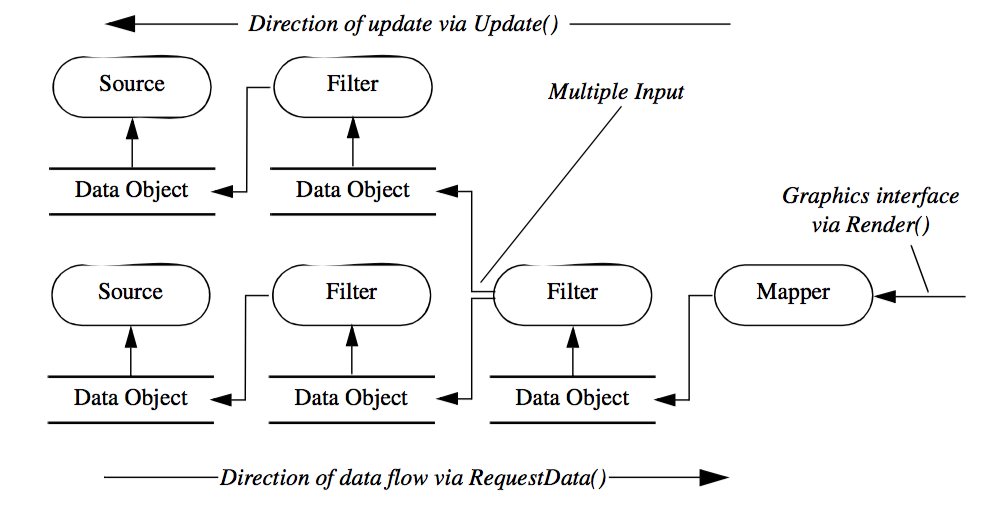
\includegraphics[width=0.8\textwidth]{Figure4-15}\\
  \caption{Description of implicit execution process implemented in VTK. The Update() method is initiated via the Render() method from the actor. Data flows back to the mapper via the RequestData() method. Arrows connecting filter and data objects indicate direction of the Update() process.}\label{fig:Figure4-15}
\end{figure}

To understand the execution of the VTK pipeline, it is useful to view the process from several different vantage points. Note that each of the following figures is not completely accurate, rather they are presented as depictions whose purpose is to describe the important features of the process.

Figure \ref{fig:Figure4-15} shows a simplified description of VTK's execution process. Generally the execution of the pipeline is triggered by a mapper's Render() method invocation, typically in response to a Render() method invocation on an associated vtkActor (which in turn receives it from the render window). Next, the Update() method is called on the input to the mapper (resulting in a cascade of method invocations requesting information and data). Eventually, data must be computed and returned to the object initiating the request, in this case the mapper. The RequestData() method actually executes the filter(s) in the pipeline and produces output data. Note the direction of flow --- here we define the direction of data flow as the \emph{downstream} direction, and the direction of the Update() invocation the \emph{upstream} direction.

\begin{figure}[!htb]
  \centering
  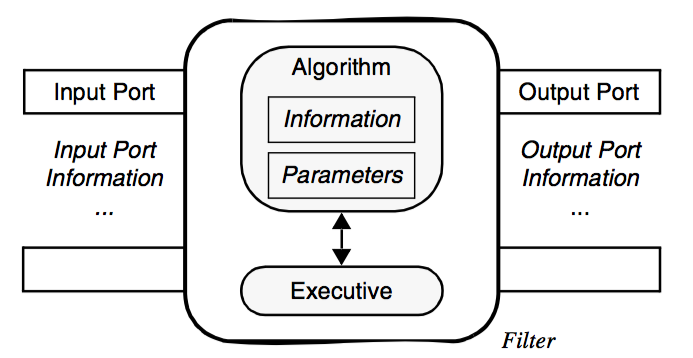
\includegraphics[width=0.8\textwidth]{Figure4-16}\\
  \caption{The logical relationship of the algorithm, executive and ports constituting a filter. The executive is responsible for managing the execution of the algorithm, and coordinating with information requests traveling through the pipeline. Ports correspond to logical, distinct inputs and outputs.}\label{fig:Figure4-16}
\end{figure}

The next figure, Figure \ref{fig:Figure4-16}, shows the relationship between the executive and the algorithm, which are paired to form a filter. This view of the filter is independent of the pipeline and contains all the information about the interface of the algorithm, namely the number and availability of inputs and outputs. Finally Figure \ref{fig:Figure4-17} shows the connections between filters. Notice that the output data object is not directly wired to the input connection. Rather the downstream filters's input connection is associated with the upstream filter's output port. This separation of data object from the input port means that data type checking can be deferred until run-time, when the consuming filter requests data from the producer of the data. Thus the producer can generate different types of data (e.g., it is a reader that produces different data types), and as long as the consumer supports these different data types, the pipeline will Qexecute without error.

\subsection{Connecting Pipeline Objects}
\label{subsec:connecting_pipeline_objects}

This leads us to the method of making connections between filters and data objects to form a visualization pipeline. As is evident from the previous figures, the \emph{Visualization Toolkit} pipeline architecture has been designed to support multiple inputs and outputs. In practice, you will find that most filters and sources actually generate a single output and filters accept a single input. This is because most algorithms tend to be single input/output in nature. There are exceptions and we will describe some of these shortly. However, first we would like to provide a brief history lesson relative to the evolution of VTK's pipeline architecture. This lesson is instructive because it sheds light on the evolution of the pipeline design in response to new requirements.

Prior to VTK 5.0. In earlier versions of VTK (i.e., prior to version 5.0), the visualization pipeline architecture was accurately depicted by Figure \ref{fig:Figure4-15}. In this figure, which shows how filters and data objects were connected to form a visualization network, the input data was represented by the Input instance variable and was set using the SetInput() method. The output data was represented by the Output instance variable and was accessed using the GetOutput()\index{GetOutput()} method. To connect filters together, the C++ statement

\begin{lstlisting}[language=C++, caption={}, numbers=none, frame=none]
filter2->SetInput(filter1->GetOutput()); //Prior to VTK5.0
\end{lstlisting}

was typically used with filter1 and filter2 filter objects of compatible type. In this design, compile time type checking was performed (i.e., the C++ compiler would enforce proper type). Obviously, this meant that correcting filters together producing output of unknown type was problematic. Several other issues with this design remained as well, many of which have been alluded to earlier, but are summarized here to motivate the use of the newer pipeline architecture. 

\begin{figure}[!htb]
  \centering
  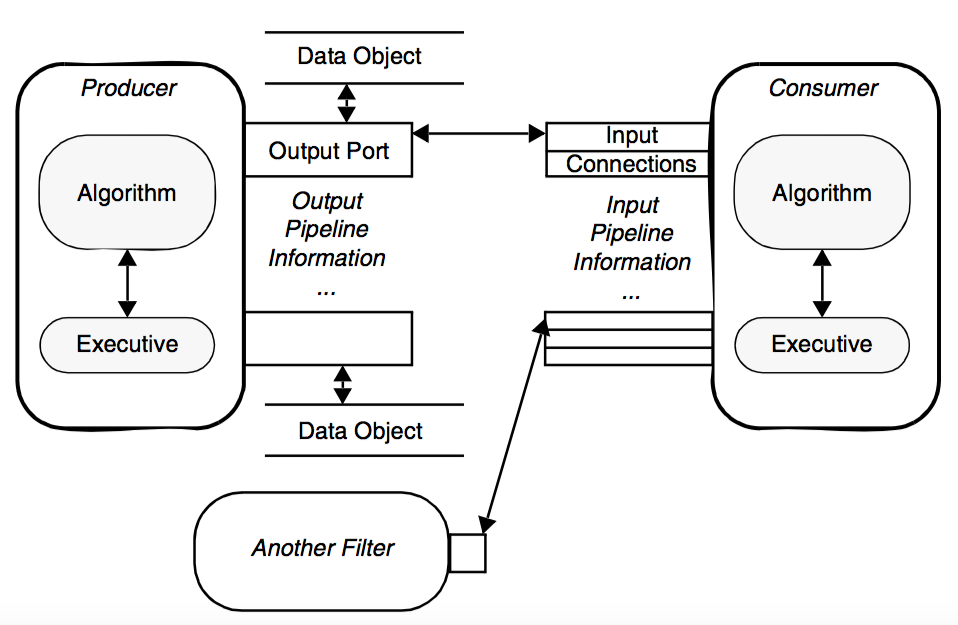
\includegraphics[width=0.8\textwidth]{Figure4-17}\\
  \caption{The logical relationship of ports and connections An input port may have more than one connection associated with it. Multiple connections are possible in certain filters such as the append filter, where a single logical input port represents all the data to be ``appended'' together, and each input is represented by a different connection.}\label{fig:Figure4-17}
\end{figure}

\begin{itemize}
\item The older design did not support deferred dataset type checking. It was difficult to support arbitrary reader types or filters that could produce different types of output.

\item The strategy for updating and managing the execution of the pipeline were implicitly embedded in the process objects and data objects. As the strategy became more complex, or needed to change, this required modifying data and/or process objects.

\item In the older design it was difficult to abort pipeline execution during an update pass. Further, it was not possible to centralize the error checking; each filter had to do some checking thereby duplicating code.

\item Introducing metadata into the pipeline required changing the API to the data and process objects. It was desirable to support the ability of a reader to add metadata to a data stream and have a filter in the pipeline retrieve it, without having to modify the API.
\end{itemize}

For this, and other reasons related to parallel processing, the original VTK pipeline design was reworked. While the transition was difficult, such changes are often necessary if a software system is to change and grow with advances in technology.

\textbf{VTK 5.0 and Beyond}. While VTK 5.0 still supports the use of SetInput()/GetOutput(), its use in Figure \ref{fig:Figure4-16} and Figure \ref{fig:Figure4-17} is discouraged. Rather, the newer pipeline architecture should be used. Referring to Figure \ref{fig:Figure4-17}, we use connections and ports to configure VTK's visualization pipeline:

\index{GetOutputPort()}

\begin{lstlisting}[language=C++, caption={}, numbers=none, frame=none]
filter2->SetInput(filter1->GetOutputPort()); // VTK5.0
\end{lstlisting}

You probably have already guessed how this approach can be extended to multiple inputs and multiple outputs. Let's look at some concrete examples. vtkGlyph3D is an example of a filter that accepts multiple inputs and generates a single output. The inputs to vtkGlyph3D are represented by the Input and Source instance variables. The purpose of vtkGlyph3D is to copy the geometry defined by the data in Source to each point defined by Input. The geometry is modified according to the Source data values (e.g., scalars and vectors). (For more information about glyphs see \nameref{subsec:glyphs} in Chapter 6: \nameref{chap:fundamental_algorithms}.) To use the vtkGlyph3D object in C++ code you would do the following:

\begin{lstlisting}[language=C++, caption={}, numbers=none, frame=none]
glyph = vtkGlyph3D::New();
glyph->SetInputConnection(foo->GetOutputPort());
glyph->SetSourceConnection(bar->GetOutputPort());
...
\end{lstlisting}

where foo and bar are filters returning the appropriate type of output. The class vtkExtractVectorComponents is an example of a filter with a single input and multiple outputs. This filter extracts the three components of a 3D vector into separate scalar components. Its three outputs are available on output ports 0, 1, and 2. An example use of the filter follows:

\begin{lstlisting}[language=C++, caption={}, numbers=none, frame=none]
vz = vtkExtractVectorComponents::New();
foo = vtkDataSetMapper::New();
foo->SetInputConnection(vz->GetOutputPort(2));
...
\end{lstlisting}

Several other special objects having multiple inputs or outputs are also available. Some of the more notable classes are vtkMergeFilter, vtkAppendFilter, and vtkAppendPolyData. These filters com bine multiple pipeline streams and generate a single output. Note, however, that while vtkMergeFilter has multiple input ports (i.e., different logical inputs), vtkAppendFilter has only one logical input, but presumes multiple connections are made to that one input. This is because in the case of vtkMergeFilter, each input has a distinct and separate purpose, while in vtkAppendFilter all the inputs have the same meaning (i.e., just one more input in a list to append together). Here are some code fragments:

\begin{lstlisting}[language=C++, caption={}, numbers=none, frame=none]
merge = vtkMergeFilter::New();
merge->SetGeometryConnection(foo->GetOutputPort());
merge->SetScalarsConnection(bar->GetOutputPort());
\end{lstlisting}

and

\begin{lstlisting}[language=C++, caption={}, numbers=none, frame=none]
append = vtkAppendFilter::New();
append->AddInputConnection(foo->GetOutputPort());
append->AddInputConnection(bar->GetOutputPort());
\end{lstlisting}

Notice the use of the method AddInputConnection()\index{AddInputConnection()}. This method adds to the list of connections, whereas SetInputConnection() clears the list and specifies the single connection to the port.

Another important filtering class is vtkProbeFilter. This filter takes two inputs. The first input is the data we wish to probe. The second input supplies a set of points that are used as probe points. Some process objects take a list of input data. Another interesting filter is the vtkBooleanStructuredPoints class which performs set operations on volume datasets. The first data item in the list is used to initialize the set operation. Each subsequent item in the list is combined with the result of previous operations using a boolean operation specified by the user.

For more details regarding the object design of filters and data objects, please see Chapter 5: \nameref{chap:basic_data_representation} and Chapter 6: \nameref{chap:fundamental_algorithms}.

\subsection{Pipeline Execution and Information Objects}
\label{subsec:pipeline_execution_and_information_objects}

Until now, we have used the terms metadata and information objects rather informally. As described previously, in the context of VTK, these terms refer to data that describes datasets. In this section, we show how these objects, which are subclasses of vtkInformation, are used to facilitate the execution of the VTK pipeline.

\begin{description}[leftmargin=0cm,labelindent=0cm]
\item[Information Objects.] Information objects are the basic containers used throughout the VTK pipeline to hold a wide variety of metadata\index{metadata}. They are heterogeneous key--to--value maps in which the type of the key determines the type of the value. The following is an enumeration of the places information objects are used.

\begin{itemize}

\item \emph{Pipeline information\index{information pipeline!objects!information}\index{information!pipeline}} objects hold information for pipeline execution. They are stored in instances of vtkExecutive or subclasses and are accessible via the method vtkExecutive::GetOutputInformation(). There is one pipeline information object per output port. It contains an entry pointing to the output vtkDataObject on the corresponding port (if it has been created). The vtkDataObject contains a pointer back to its corresponding pipeline information object, accessible via vtkDataObject::GetPipelineInformation(). The pipeline information object also holds information about what will populate the data object when the filter executes and generates the output. The actual information contained is determined by the output data type and the execution model in use. Pipeline information objects for input connections are accessible via the method vtkExecutive::GetInputInformation(), and they are the pipeline information objects on the output ports to which the input ports are connected.

\item \emph{Port information\index{information!port}} objects hold information about the data types produced on output ports and consumed by input ports. They are stored by instances of vtkAlgorithm. There is one input port information object per input port and one output port information object per output port. They are accessible via the methods vtkAlgorithm::GetInputPortInformation() and vtkAlgorithm::GetOutputPortInformation(). Port information objects are usually created and populated by subclasses of vtkAlgorithm in order to specify the interface of the filter.

\item \emph{Request information\index{information!request}} objects hold information about a specific request being sent to an executive or algorithm. There is one entry indicating what request is being sent and possibly other entries giving additional details about the specific request. These information objects are not accessible via any public method but are passed to ProcessRequest() methods that implement the requests.

\item \emph{Data information\index{data information}\index{information!data}} objects hold information about what is currently stored in a vtkDataObject. There is one data information object in each data object, accessible via vtkDataObject::GetInformation(). The actual information contained is determined by the data object type.

\item \emph{Algorithm information\index{algorithm information}\index{information!algorithm}} objects hold information about an instance of vtkAlgorithm. There is one algorithm information object per algorithm object, accessible via vtkAlgorithm::GetInformation(). The actual information contained is determined by the algorithm object type.
\end{itemize}

The importance of the information objects in VTK is that they are flexible (e.g., new key-value pairs can be easily added) and extensible. That is, readers, filters and mappers can add new information to the containers without requiring the API of the pipeline--related classes to change.

\begin{figure}[!htb]
  \centering
  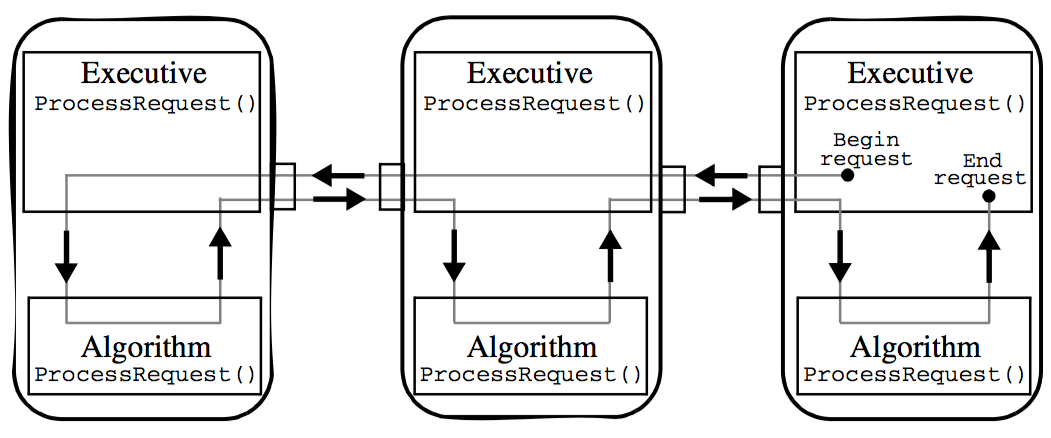
\includegraphics[width=0.8\textwidth]{Figure4-18}\\
  \caption{Path of a request sent through a pipeline. For example, assume the consumer (at the far right) needs only a single piece of this data (e.g., piece 1 of 4); also assume that the producer (on the far left) is a reader that can partition its data into pieces. The consumer passes this request upstream, and it continues upstream (via executives) until it reaches a producer that can fulfill the request. When the reader algorithm is asked for a piece of the data, it provides it, and passes the new data back (with the information that it is piece 1 of 4) down the pipeline. It stops when it reaches the consumer who made the request.}\label{fig:Figure4-18}
\end{figure}

\item[Pipeline Execution Models]
\label{subsubsec:pipeline_execution_models}

In VTK, the fundamental pipeline update mechanism is based on the request. A request is the basic pipeline operation (or ``pipeline pass'') that generally asks for particular piece of information to be propagated through the pipeline. An execution model is a set of requests defined by a specific executive. Refer to Figure \ref{fig:Figure4-18} in the following description of the execution process.

Requests are generated by the executive object of a filter that has been explicitly asked to update by its algorithm due to some user call. For example, when the Write() method of a writer is called, the algorithm object asks its executive to update the pipeline, and execute the writer, by calling this->GetExecutive()->Update(). Several requests may be sent through the pipeline in order to bring it up to date.

A request is implemented as an information object. There is one key of type vtkInformationRequestKey specifying the request itself. This key is typically defined by the executive's class. Additional information about the request may also be stored in the request information object.
       
Requests are propagated through the pipeline by the executives of each filter. The vtkExecutive::ProcessRequest() method is invoked on an executive given the request information object. This method is implemented by each executive and is responsible for fulfilling the request as it sees fit. Many requests may be fulfilled for a filter only after it has been fulfilled for the filters providing its inputs. For these requests the executive will pass the request on to the executives of these upstream filters and then handle the request itself.

An executive often asks its algorithm object for help in fulfilling a request. It sends the request to the algorithm object by invoking the vtkAlgorithm::ProcessRequest() method. This method is implemented by all algorithms and is responsible for handling the request. Input and output pipeline information objects are provided as arguments to the method. The algorithm must handle the request using only its own filter parameter settings and the pipeline information objects given. An algorithm is not allowed to ask its executive for any additional information. This insures that the algorithms are independent of the executives. Figure \ref{fig:Figure4-18} shows a typical path taken by a request as it is sent through a pipeline. Typically the request originates in a consumer at the end of the pipeline. It is sent back through the pipeline by the executives. Each executive asks its algorithm to help handle the request.
\end{description}

\subsection{Flexible Computation / Memory Trade-off}
\label{subsec:flexible_computation_memory_trade-off}

By default, networks constructed using the \emph{Visualization Toolkit} store intermediate computational results (i.e., favor computation). However, a single class variable can be set to discard intermediate data when they are no longer needed (i.e., favor memory). In addition, a local parameter can be set within each process object to control this trade-off at object level.

This global variable is set as follows. Given the data object O, (or the output of a filter obtained using O=filter->GetOutput()), invoke O->SetGlobalReleaseDataFlagOn() to enable data release. To enable data release for a particular object use O->SetReleaseDataFlagOn(). Appropriate methods exist to disable memory release as well.

\subsection{High-Level Object Design}
\label{subsec:high-level_object_design}

At this point in the text it is premature to describe design details of the various objects making up the visualization pipeline. However, there are two important classes that affect many of the objects in the text. These are the classes vtkObject and vtkObjectBase.

vtkObjectBase is the base object for almost all inheritance hierarchies found in VTK. vtkObjectBase implements data object reference counting (see ``Reference Counting and Garbage Collection'' on page \pageref{subsec:reference_counting_garbage_collection}). Subclasses of vtkObjectBase may be shared by other objects, without duplicating memory. It also defines an API for objects to print information about themselves.

vtkObject is a subclass of vtkObjectBase. It provides methods and instance variables to control run-time debugging and maintains internal object modification time. In particular, the method Modified() is used to update the modification time, and the method GetMTime() is used to retrieve it. vtkObject also provides a framework for the event callbacks that we saw in the previous chapter (see ``Events and Observers''on page \pageref{sub:examples_events_observers}).

Note that we do not always include vtkObject and vtkObjectBase in object diagrams to conserve space. Refer to the source code for a definitive statement.

\subsection{Examples}
\label{subsec:Ch04Examples}

We will now demonstrate some of the features of the visualization pipeline with four examples. Some of the objects used here will be unfamiliar to you. Please overlook missing details until we cover the information later in the book. The goal here is to provide a flavor and familiarity with the software architecture and its use.

\subsubsection{Simple Sphere}
\label{subsubsec:simple_sphere}

The first example demonstrates a simple visualization pipeline. A polygonal representation of a sphere is created with the source object (vtkSphereSource). The sphere is passed through a filter (vtkElevationFilter) that computes the height of each point of the sphere above a plane. The plane is perpendicular to the z-axis, and passes through the point (0,0,-1). The data is finally mapped (vtkDataSetMapper) through a lookup table. The mapping process converts height value into colors, and interfaces the sphere geometry to the rendering library. The mapper is assigned to an actor, and then the actor is displayed. The visualization network, a portion of code, and output image are shown in Figure \ref{fig:Figure4-19}.

The execution of the pipeline occurs implicitly when we render the actor. Each actor asks its mapper to update itself. The mapper in turn asks its input to update itself. This process continues until a source object is encountered. Then the source will execute if modified since the last render.

\begin{figure}[htb]
    \centering
    \begin{subfigure}[h]{0.96\linewidth}
        \begin{subfigure}[h]{0.48\linewidth}
        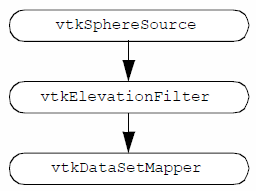
\includegraphics[width=0.96\linewidth]{Figure4-19a}
        \caption*{}
        \label{fig:Figure4-19a}
        \end{subfigure}
        \hfill
        \begin{subfigure}[h]{0.48\linewidth}
        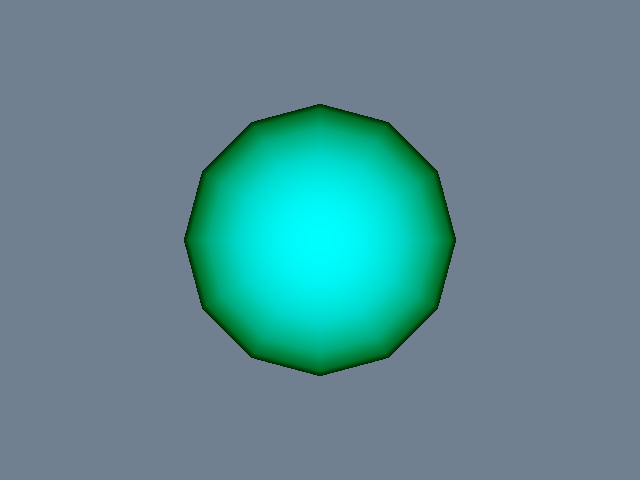
\includegraphics[width=0.96\linewidth]{Figure4-19b}
        \caption*{See: href{https://lorensen.github.io/VTKExamples/site/Cxx/Rendering/ColoredSphere/}{ColoredSphere.cxx} and \href{https://lorensen.github.io/VTKExamples/site/Python/Rendering/ColoredSphere/}{ColoredSphere.py}.})
        \label{fig:Figure4-19b}
        \end{subfigure}
  \end{subfigure}
  \hfill
  \begin{subfigure}[h]{0.76\linewidth}{Figure4-19c}
  \begin{lstlisting}[language=C++,  caption={}, numbers=none, frame=none]
    vtkSphereSource *sphere = vtkSphereSource::New();
      sphere->SetPhiResolution(12); sphere->SetThetaResolution(12);
    
    vtkElevationFilter *colorIt = vtkElevationFilter::New();
      colorIt->SetInputConnection(sphere->GetOutputPort());
      colorIt->SetLowPoint(0,0,-1);
      colorIt->SetHighPoint(0,0,1);
    
    vtkDataSetMapper *mapper = vtkDataSetMapper::New();
      mapper->SetInputConnection(colorIt->GetOutputPort());
      
    vtkActor *actor = vtkActor::New();
      actor->SetMapper(mapper);
    \end{lstlisting} 
    \caption*{}
  \end{subfigure}
  \caption{A simple sphere example.}\label{fig:Figure4-19}
\end{figure}

Then the system walks through the network and executes each object if its input or instance variables are out of date. When completed, the actor's mapper is up to date and an image is generated.

Now let's reexamine the same process of pipeline execution by following method invocation. The process begins when the actor receives a Render() message from a renderer. The actor in turn sends a Render() message to its mapper. The mapper begins network execution by asking its input to update itself via the Update() operation. This causes a cascade of Update() methods as each filter in turn asks its input to update itself. If branching in the pipeline is present, the update method will branch as well. Finally, the cascade terminates when a source object is encountered. If the source object is out of date, it will send itself an RequestData() command. Each filter will send itself an RequestData() as necessary to bring itself up to date. Finally, the mapper will perform operations to transform its input into rendering primitives.

In the \emph{Visualization Toolkit}, the Update() method is public while the RequestData() method is protected. Thus, you can manually cause network execution to occur by invoking the Update() operation. This can be useful when you want to set instance variables in the network based on the results of upstream execution, but do not want the whole network to update. The RequestData() method is protected because it requires a certain object state to exist. The Update() method insures that this state exists.

One final note. The indentation of the code serves to indicate where objects are instantiated and modified. The first line (i.e., the New() operator) is where the object is created. The indented lines that follow indicate that various operations are being performed on the object. We encourage you to use a similar indenting scheme in your own work.

\subsubsection{Warped Sphere}
\label{subsubsec:warped_sphere}

This example extends the pipeline of the previous example and shows the effects of type checking on the connectivity of process objects. We add a transform filter (vtkTransformFilter) to nonuniformly scale the sphere in the x-y-z directions.

The transform filter only operates on objects with explicit point coordinate representation (i.e., a subclass of vtkPointSet). However, the elevation filter generates the more general form vtkDataSet as output. Hence we cannot connect the transform filter to the elevation filter. But we can connect the transform filter to the sphere source, and then the elevation filter to the transform filter. The result is shown in Figure \ref{fig:Figure4-20}. (Note: an alternative method is to use vtkCastToConcrete to perform run-time casting.)

The C++ compiler enforces the proper connections of sources, filters, and mappers. To decide which objects are compatible, we check the type specification of the SetInput() method. If the input object returns an output object or a subclass of that type, the two objects are compatible and may be connected.

\begin{figure}[htb]
    \centering
    \begin{subfigure}[h]{0.96\linewidth}
      \begin{subfigure}[h]{0.48\linewidth}
        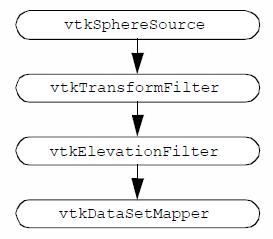
\includegraphics[width=0.96\linewidth]{Figure4-20a}
        \caption*{}
        \label{fig:Figure4-20a}
      \end{subfigure}
      \hfill
      \begin{subfigure}[h]{0.48\linewidth}
        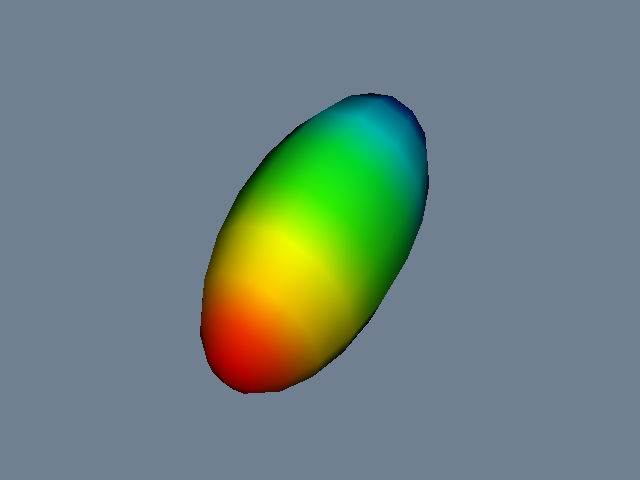
\includegraphics[width=0.96\linewidth]{Figure4-20b}
        \caption*{(\href{https://lorensen.github.io/VTKExamples/site/Cxx/Rendering/TransformSphere/}{TransformSphere.cxx} or \href{https://lorensen.github.io/VTKExamples/site/Python/Rendering/TransformSphere/}{TransformSphere.py}).}
        \label{fig:Figure4-20b}
      \end{subfigure}
  \end{subfigure}
  \hfill
  \begin{subfigure}[h]{0.76\linewidth}
    \begin{lstlisting}[language=C++, caption={Warped Sphere.}]
    vtkSphereSource *sphere = vtkSphereSource::New();
      sphere->SetThetaResolution(12);
      sphere->SetPhiResolution(12);

    vtkTransform *aTransform = vtkTransform::New();
      aTransform->Scale(1,1.5,2);

    vtkTransformFilter *transFilter = vtkTransformFilter::New();
      transFilter->SetInputConnection(sphere->GetOutputPort());
      transFilter->SetTransform(aTransform);

    vtkElevationFilter *colorIt = vtkElevationFilter::New();
      colorIt->SetInputConnection(transFilter->GetOutputPort());
      colorIt->SetLowPoint(0,0,-1);
      colorIt->SetHighPoint(0,0,1);

    vtkLookupTable *lut = vtkLookupTable::New();
      lut->SetHueRange(0.667,0.0); lut->SetSaturationRange(1,1);
      lut->SetValueRange(1,1);

    vtkDataSetMapper *mapper = vtkDataSetMapper::New();
      mapper->SetLookupTable(lut);
      mapper->SetInputConnection(colorIt->GetOutputPort());

    vtkActor *actor = vtkActor::New();
      actor->SetMapper(mapper);
    \end{lstlisting}
    \caption*{}
    \label{fig:Figure4-20c}
  \end{subfigure}
  \caption{The addition of a transform filter to the previous example.}\label{fig:Figure4-20}
\end{figure}

\subsubsection{Generating Oriented Glyphs}
\label{subsubsec:generating_oriented_glyphs}

This example demonstrates the use of an object with multiple inputs. vtkGlyph3D places 3D icons or glyphs (i.e., any polygonal geometry) at every input point. The icon geometry is specified with the instance variable Source, and the input points are obtained from the Input instance variable. Each glyph may be oriented and scaled in a variety of ways, depending upon the input and instance variables. In our example we place cones oriented in the direction of the point normals (Figure \ref{fig:Figure4-21}).

The visualization network branches at vtkGlyph3D. If either branch is modified, then this filter will reexecute. Network updates must branch in both directions, and both branches must be up to date when vtkGlyph3D executes. These requirements are enforced by the Update() method, and pose no problem to the implicit execution method.

\begin{figure}[htb]
  \begin{subfigure}[h]{0.64\linewidth}
    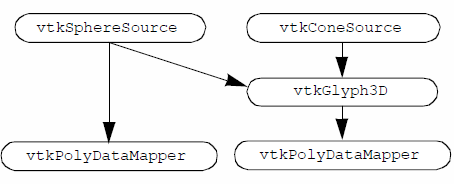
\includegraphics[width=0.96\linewidth]{Figure4-21a}
    \caption*{}
    \label{fig:Figure4-21a}
  \end{subfigure}
  \hfill
  \begin{subfigure}[h]{0.32\linewidth}
    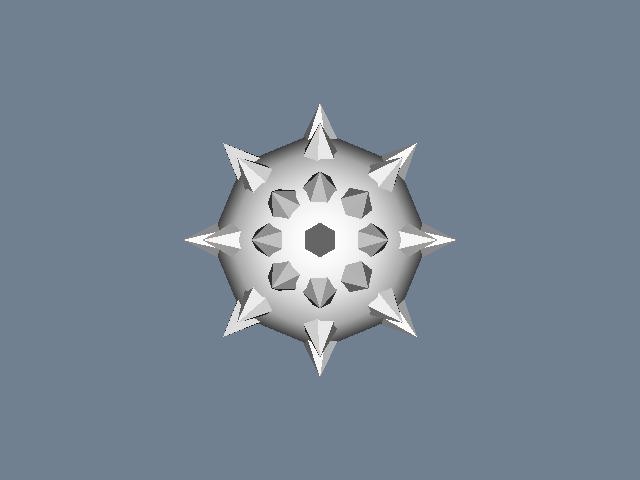
\includegraphics[width=0.96\linewidth]{Figure4-21b}
    \caption*{See: \href{https://lorensen.github.io/VTKExamples/site/Cxx/Rendering/Mace/}{Mace.cxx} and \href{https://lorensen.github.io/VTKExamples/site/Python/Rendering/Mace/}{Mace.py}.}
    \label{fig:Figure4-21b}
  \end{subfigure}
  \hfill
  \begin{subfigure}[h]{0.96\linewidth}{Figure4-22c}
    \begin{lstlisting}[language=C++, caption={Warped Sphere.}]
    vtkSphereSource *sphere = vtkSphereSource::New();
      sphere->SetThetaResolution(8); sphere->SetPhiResolution(8);
    
    vtkPolyDataMapper *sphereMapper = vtkPolyDataMapper::New();
      sphereMapper->SetInputConnection(sphere->GetOutputPort());
    
    vtkActor *sphereActor = vtkActor::New();
      sphereActor->SetMapper(sphereMapper);
    
    vtkConeSource *cone = vtkConeSource::New();
      cone->SetResolution(6);
    
    vtkGlyph3D *glyph = vtkGlyph3D::New();
      glyph->SetInputConnection(sphere->GetOutputPort());
      glyph->SetSourceConnection(cone->GetOutputPort());
      glyph->SetVectorModeToUseNormal();
      glyph->SetScaleModeToScaleByVector();
      glyph->SetScaleFactor(0.25);
    
    vtkPolyDataMapper *spikeMapper = vtkPolyDataMapper::New();
      spikeMapper->SetInputConnection(glyph->GetOutputPort());
    
    vtkActor *spikeActor = vtkActor::New();
      spikeActor->SetMapper(spikeMapper);
    \end{lstlisting}
    \caption*{}
  \end{subfigure}
  \caption{An example of multiple inputs and outputs.}\label{fig:Figure4-21}
\end{figure}

\textbf{Disappearing Sphere}. In our last example we construct a visualization network with a feedback loop, and show how we can use procedural programming to change the topology of the network. The network consists of four objects: vtkSphereSource to create an initial polygonal geometry, vtkShrinkFilter to shrink the polygons and create a gap or space between neighbors, vtkElevationFilter to color the geometry according to height above the x-y plane, and vtkDataSetMapper to map the data through a lookup table and interface to the rendering library. The network topology, a portion of the C++ code, and output are shown in Figure \ref{fig:Figure4-22}.

After vtkSphereSource generates an initial geometry (in response to a render request), the input of vtkShrinkFilter is changed to the output of the vtkElevationFilter. Because of the feedback loop, vtkShrinkFilter will always reexecute. Thus, the behavior of the network is to reexecute each time a render is performed. Because the shrink filter is reapplied to the same data, the polygons become smaller and smaller and eventually disappear.

\begin{figure}[htb]
  \begin{subfigure}[h]{0.48\linewidth}
    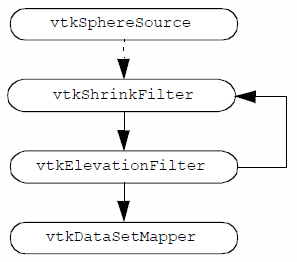
\includegraphics[width=0.96\linewidth]{Figure4-22a}
    \caption*{}
    \label{fig:Figure4-22a}
  \end{subfigure}
  \hfill
  \begin{subfigure}[h]{0.48\linewidth}
    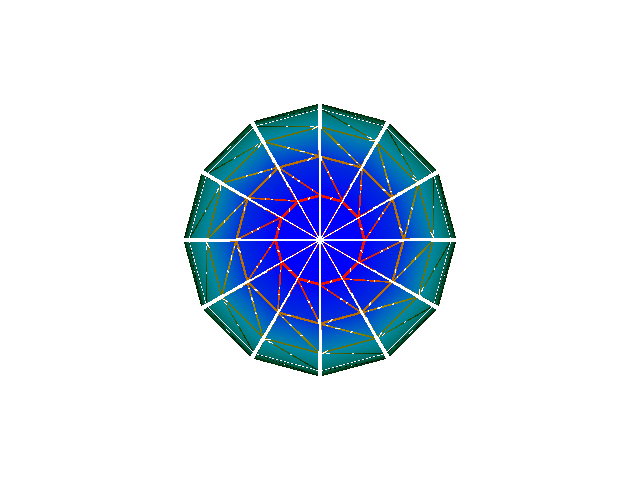
\includegraphics[width=0.96\linewidth]{Figure4-22b}
    \caption*{See: \href{https://lorensen.github.io/VTKExamples/site/Cxx/Visualization/LoopShrink/}{LoopShrink.cxx} and \href{https://lorensen.github.io/VTKExamples/site/Python/Visualization/LoopShrink/}{LoopShrink.py}.}
    \label{fig:Figure4-22b}
  \end{subfigure}
  \hfill
  \begin{subfigure}[h]{0.96\linewidth}{Figure4-22c}
    \begin{lstlisting}[language=C++, caption={Warped Sphere.}]
    vtkSphereSource *sphere = vtkSphereSource::New();
      sphere->SetThetaResolution(12); sphere->SetPhiResolution(12);
    
    vtkShrinkFilter *shrink = vtkShrinkFilter::New();
      shrink->SetInputConnection(sphere->GetOutputPort());
      shrink->SetShrinkFactor(0.9);
    
    vtkElevationFilter *colorIt = vtkElevationFilter::New();
      colorIt->SetInputConnection(shrink->GetOutputPort());
      colorIt->SetLowPoint(0,0,-.5);
      colorIt->SetHighPoint(0,0,.5);
    
    vtkDataSetMapper *mapper = vtkDataSetMapper::New();
      mapper->SetInputConnection(colorIt->GetOutputPort());
    
    vtkActor *actor = vtkActor::New();
      actor->SetMapper(mapper);
    
      renWin->Render(); // execute first time
      // create loop
      shrink->SetInputConnection(colorIt->GetOutputPort());
      renWin->Render(); // begin looping
    \end{lstlisting}
    \caption*{}
  \end{subfigure}
  \caption{A network with a loop (LoopShrk.cxx). VTK 5.0 does not allow you to execute a looping visualization network; this was possible in previous versions of VTK.}\label{fig:Figure4-22}
\end{figure}

\section{Chapter Summary}
\label{Ch04ChapterSummary}

The visualization process is naturally modelled using a combination of functional and object models. The functional model can be simplified and used to describe visualization networks. The object model specifies the components of the visualization network. Visualization networks consist of process objects and data objects. Data objects represent information; process objects transform the data from one form to another. There are three types of process objects --- sources have no input and at least one output; filters have at least one input and output; sinks, or mappers, terminate the visualization network. The execution of the network can be controlled implicitly or explicitly. Implicit control means that each object must insure its input is up to date, thereby distributing the control mechanism. Explicit control means that there is a centralized executive to coordinate the execution of each object. Many techniques are available to program visualization networks. Direct visual programming is most common in commercial systems. At a higher level, applications provide tailored but more rigid interfaces to visualize information. At the lowest level, subroutine or object libraries provide the greatest flexibility. The \emph{Visualization Toolkit} contains an object library implemented in C++ for constructing visualization networks.

\section{Bibliographic Notes}
\label{Ch04BibNotes}

The practical way to learn about the visualization process is to study commercially available systems. These systems can be categorized as either direct visual programming environments or as applications. Common visual programming systems include AVS\index{AVS} \cite{AVS89}, Iris Explorer\index{Iris Explorer} \cite{IrisExplorer}, IBM Data Explorer\index{Data Explorer} \cite{DataExplorer}, apE\index{apE} \cite{apE90}, and Khoros\index{Khoros} \cite{Rasure91}. Application systems generally provide less flexibility than visual programming systems, but are better tailored to a particular problem domain. PLOT3D \cite{PLOT3D} is an early example of a tool for CFD visualization. This has since been superseded by FAST\index{FAST} \cite{FAST90}. FieldView\index{FieldView} is another popular CFD visualizer \cite{FieldView91}. VISUAL3 \cite{VISUAL3} is a general tool for unstructured or structured grid visualization. PV-WAVE\index{PV-WAVE} \cite{Charal90} can be considered a hybrid system, since it has both simple visual programming techniques to interface to data files as well as a more structured user-interface than the visual programming environments. Wavefront's Data Visualizer\index{Data Visualizer} \cite{DataVisualizer} is a general--purpose visualization tool. It is unique in that it is part of a powerful rendering and animation package. A nice system for visualizing 3D gridded data (such as that produced by numerical weather models) is VIS5D. Find out more at the \href{http://www.ssec.wisc.edu/\~billh/vis5d.html}{VIS5D Web site}).

Although many visualization systems claim to be object--oriented, this is often more in appearance than implementation. Little has been written on object--oriented design issues for visualization. \cite{VISAGE92} presents an architecture similar to that described in this chapter. Favre \cite{Favre94} describes a more conventional object--oriented approach. His dataset classes are based on topological dimension and both data and methods are combined into classes.

\printbibliography

\section{Exercises}
\begin{enumerate}

\item Consider the following 2D visualization techniques: $x-y$ plotting, bar charts, and pie charts.

For each technique:

\begin{enumerate}

    \item Construct functional models.

    \item Construct object models.

\end{enumerate}

    \item \label{ex:ch04_4.2} A \emph{height field}\index{height field} is a regular array of 2D points where $h = f(x,y)$, $h$ is an altitude above the point $(x,y)$. Height fields are often used to represent terrain data. Design an object--oriented system to visualize height fields.

\begin{enumerate}

    \item How would you represent the height field?

    \item What methods would you use to access this data?

    \item Develop one process object (i.e., visualization technique) to visualize a height field. Describe the methods used by the object to access and manipulate the height field.

\end{enumerate}

\item Describe how you would implement an explicit control mechanism for network execution.

\begin{enumerate}

    \item How do process objects register their input data with the executive?

    \item How is the executive notified of object modification?

    \item By what method is the executive notified that network execution is necessary?

    \item Describe an approach for network dependency analysis. How does the executive invoke execution of the process objects?

\end{enumerate}

\item Visual programming environments enable the user to construct visualization applications by graphically connecting process objects.

\begin{enumerate}

    \item Design a graphical notation to represent process objects, their input and output, and data flow direction.

    \item How would you modify instance variables of process objects (using a graphical technique)?

    \item By what mechanism would network execution be initiated?

    \item How would you control conditional execution and looping in your network?

    \item How would you take advantage of parallel computing?

    \item How would you distribute network execution across two or more computers sharing a network connection?

\end{enumerate}

\item Place oriented cylinders (instead of cones) on the mace in Figure \ref{fig:Figure4-20}. (\emph{Hint}: use vtkCylinderSource.)

\item The implicit update method for the visualization network used by VTK is simple to implement and understand. However, it is prone to a common programming error. What is this error?

\item Experiment with the transformation object in Figure \ref{fig:Figure4-20}.

\begin{enumerate}

    \item Translate the actor with vtkTransform's Translate() method.

    \item Rotate the actor with the RotateX(), RotateY(), and RotateZ() methods.

    \item Scale the actor with the Scale() method.

    \item Try combinations of these methods. Does the actor transform in ways that you expect?

\end{enumerate}

\item Visualize the following functions. (\emph{Hint}: use vtkSampleFunction and refer to Figure \ref{fig:Figure4-1}.)

\begin{enumerate}

    \item $F(x,y,z)=x^2$

    \item $F(x,y,z) = x_2 + 2 y + 3 z +1$

    \item $F(x,y,z) = x+2 + y^2 - \cos (z) + 1$

\end{enumerate}

\end{enumerate}

